\documentclass{l4proj}

\usepackage{url}
\usepackage{fancyvrb}
\usepackage[final]{pdfpages}
\usepackage{hyperref}
\usepackage{fancyvrb}
\usepackage{float}
\usepackage{multirow}
\usepackage{graphicx}
\usepackage{amsmath}
\usepackage{MnSymbol}
\usepackage{wasysym}
\usepackage{mathtools}
\usepackage{subcaption}
\usepackage{relsize}
\usepackage{algorithm}
\usepackage[noend]{algpseudocode}
\usepackage{listings}
\usepackage[utf8]{inputenc}
\usepackage{fancybox}
\usepackage{chngcntr}
\usepackage[toc,page]{appendix}

\counterwithout{footnote}{chapter}

\lstset{
  basicstyle=\ttfamily,
  mathescape
}

\hypersetup{
    colorlinks,
    citecolor=black,
    filecolor=black,
    linkcolor=black,
    urlcolor=black
}

\makeatletter
\newenvironment{CenteredBox}{
\begin{Sbox}}{
\end{Sbox}\centerline{\parbox{\wd\@Sbox}{\TheSbox}}}
\makeatother


\makeatletter
\def\BState{\State\hskip-\ALG@thistlm}
\makeatother

\begin{document}
\title{Implementations of Advanced K-Means Clustering Algorithms \\ for Spark/MLlib}
\author{Ivan Kyosev}
\date{March 21, 2017}
\maketitle

\begin{abstract}
Apache Spark is a fast and general engine for large-scale data processing. It emphasizes speed, ease of use and generality in regards to working with Big Data. Its feature-set provides an alternative to the popular Hadoop MapReduce software framework, displaying a noticeable performance improvement. One of Spark's many components is MLlib. It is a machine learning library built on top of the core features of Spark and provides implementations for a variety of popular machine learning algorithms, written in a way meant to support scalability when operating on big data sets.

This paper presents a proposed extension to the MLlib component of Apache Spark in the form of additional K-Means Clustering algorithms that the library does not currently support. K-Means clustering is a method of vector quantization, originally from signal processing, that is popular for cluster analysis in data mining. A thorough analysis of the performance of the newly created algorithms and the relative quality of the produced data models is also conducted.
\end{abstract}

\renewcommand{\abstractname}{Acknowledgements}
\begin{abstract}
I would like to thank Dr. Nikos Ntarmos and Dr. Christos Anagnostopoulos for supervising this project and providing me with continuous feedback and assistance.
\end{abstract}

\educationalconsent

\tableofcontents

\chapter{Introduction}
\label{intro}
\pagenumbering{arabic}

Machine learning is an increasingly popular and relevant part of modern day systems looking to extract knowledge and value from the world around them. It refers to an approach to computation, where applications can learn without being explicitly programmed. These kinds of apps can analyze a provided sample of data and make predictions or decisions, based on some form of discovered pattern or correlation between the individual elements of the input set.

By being able to take rational choices, through examining the surrounding environment, systems that employ machine learning have become a central component of artificial intelligence. Because these system adapt their behavior based on new ``experiences'' they are utilized in a wide range of computing tasks, where developing explicit algorithms is not feasible. Such examples include solving problems in speech recognition, vision and robotics.

These machine learning algorithms are typically classified into three different categories based on the nature of the data they are learning from and the feedback of information for each input item:

\begin{itemize}
\item Supervised learning - in this case a program presented with a particular input set of data is also given the desired output, with the end goal of having the machine learn a mapping function from inputs to outputs
\item Unsupervised learning - here the elements of the input data set are not provided with a desired output value in pairs, so the system is left on its own to find structure in its input
\item Reinforcement learning - this refers to the idea of having an program interact with a dynamic environment, where it is attempting to achieve a certain goal. Along with every action, the program is also provided with positive or negative feedback, depending on whether the action aided in achieving the goal or not. 
\end{itemize}

Many of these machine learning algorithms have a similar underlying approach to their implementation. Input training data with some unknown probability distribution is presented and the program has to construct a model that allows it to extract meaning from the data and make sufficiently accurate predictions for instances that have not been encountered yet. This is generally achieved by defining a loss function and adjusting the model in attempts to minimize this loss with respect to the inputs -- effectively an optimization problem.

It is clear that machine learning algorithms heavily depend on the availability of input data in order to optimize their models to more accurately reflect the state of the real world. Therefore the quantity of supplied input data begins to have a significant impact on the quality of the output produced by application relying on machine learning. With the advent of big data and technologies meant to enable fast and reliable processing of big data, these algorithms can now make use of vast amounts of information, enabling them to create more accurate and valuable results. Examples of big data processing frameworks include Hadoop and Apache Spark.

The Apache Spark project in particular includes a component called MLlib. MLlib is a machine learning library built on top of the core features of Spark. It provides implementations for a variety of popular machine learning algorithms, all of which are written in a way meant to support horizontal scalability\footnote{Horizontal scaling refers to the scaling of a system by adding more parallel, similar in performance nodes. It is directly contrasted by vertical scaling where additional resources are added to the one node of a system.} when operating on big data sets.

\section{Aims}

The aim of this project is to create an extension to the MLlib component of Apache Spark, by developing implementations for a variety of K-Means clustering algorithms that the framework does not currently support. The newly introduced algorithms also need to be evaluated and contrasted with the ones already provided by Spark.

K-Means clustering is an example of an unsupervised machine learning algorithm. It is a method of vector quantization\footnote{Quantization is the process of mapping a large set of input values to a smaller set.}, that originated from signal processing. Its primary purpose is to group a collection of \texttt{N} data points into \texttt{K} distinct clusters. There is a variety of algorithms that produce the end result of grouping data points into \texttt{K} clusters, with varying levels of speed and accuracy. The ones that this project aims to implement as part of Spark could deliver a desired performance improvement with minimal loss in quality.

\section{Report outline}

The remainder of this report will focus on the mathematics underlying each of the considered K-Means clustering algorithms as well as the challenges of implementing them in a scalable fashion under Spark:
\begin{itemize}
\item \textbf{Chapter~\ref{spark}} covers the data processing model provided by Apache Spark and its machine learning library MLlib
\item \textbf{Chapter~\ref{kmeans}} explains the most common used versions of K-Means Clustering algorithms
\item \textbf{Chapter~\ref{previous}} discusses the approach taken by Spark's developers to create the current clustering API
\item \textbf{Chapter~\ref{propose}} outlines the proposed algorithms to be implemented as part of Apache Sparks, along with their benefits and challenges
\item \textbf{Chapter~\ref{online}} details two different approaches to the implementation of Lloyd's Online K-Means Clustering algorithm
\item \textbf{Chapter~\ref{art}} presents a version of K-Means using Adaptive Resonance Theory and its implementation
\item \textbf{Chapter~\ref{som}} presents the implementation of a  a K-Means Clustering algorithm using Self-Organizing Maps
\item \textbf{Chapter~\ref{eval}} covers a variety of ways to evaluate both the performance of the presented algorithms and the quality of the data models they produce
\item \textbf{Chapter~\ref{conclusion}} concludes this report with a reflection on the whole project
\end{itemize}

%==============================================================================

\chapter{Introduction to Apache Spark and MLlib}
\label{spark}
\section{Apache Spark}

A new big data processing paradigm in the form of cluster computing has become widely popular in recent years. It is a model where data-parallel computations are executed on clusters of unreliable machines by systems that provide scheduling, fault tolerance and load balancing\cite{Spark}. Hadoop MapReduce was the first software framework to implement these principles\cite{MapReduce}, with systems like Dryad\cite{Dryad} and Map-Reduce-Merge\cite{MRM} generalizing the supported types of data flows. These system achieve fault tolerance and scalability by supplying the user with a means of expressing computation as an acyclic data flow graph which passes the input data through a set of operations. This enables the underlying system to handle any occurring faults as well as scheduling without any user interaction.

Apache Spark is one of the latest big data processing frameworks which implements the cluster computing model. One of its primary advantages over Hadoop is that it can perform in-memory data processing, while Map-Reduce persists all outputs back to disk after a map or reduce action. This extends the scope of problems which can be solved efficiently by Spark to also include applications that reuse a working set of data across multiple parallel operations. It is impractical to implement these kinds of apps under Hadoop as between each iteration of an algorithm over the working set, the job must reload the data from disk, causing unnecessary overhead, resulting in degraded performance. Examples include iterative jobs and interactive analysis\cite{Spark}.

Due to its differences in design philosophy, users of the Spark framework have reported a 100x speed increase in certain work loads, versus a similar MapReduce solution, as well as a 10x faster execution on disk\cite{webSpark}. This performance improvement, however, results in the system requiring more RAM to carry out its operations.

The core components of Spark are implemented in Scala - a statically typed functional programming language that runs on top of the Java Virtual Machine. It also includes object-oriented features and supports Java interoperability thanks to its JVM roots -- this allows Spark to easily interact with Java based systems such as HDFS. In addition to Scala the framework also export an API available in Java, Python and R.

Spark can also be used interactively from a modified version of the Scala interpreter. This method provides full access to the API, allowing a user to define variables, functions, classes and run parallel jobs on a computer cluster. Spark is possibly the first system that allows a general-purpose programming language to be used interactively to process large data sets on a cluster\cite{Spark}.

\section{Resilient Distributed Datasets}

To achieve its goals, Spark introduces an abstraction called resilient distributed datasets -- RDDs. They are a parallel, fault-tolerant data structure that lets users explicitly persist intermediate results in memory, control their partitioning to optimize data placement, and manipulate them using a rich set of operations\cite{RDD}. The RDD API is the primary way of expressing computation on big data sets in Apache Spark.

\subsection{Basics of the RDD API}

An RDD is a read-only partitioned collection of records. It supports a series of methods that resemble operations, available to most collections in a functional programming language\footnote{Despite the nature of the RDD based API, code written in Spark does not need to adhere to the principles of pure functional programing.}. RDDs can only be created through deterministic operations on either data in stable storage or other RDDs. Such functions are known as transformations -- examples include \textit{map}, \textit{filter}, \textit{flatMap} and others. Transformations are lazy\footnote{A lazy function is not evaluated when it is called, but rather when something else tries to access its result.} operations that define a new RDD, which is typically the result of applying the same function to every data item in the source RDD -- making Spark ideal for batch processing. By chaining together several of these transformations a user can define a directed acyclic graph (DAC) of operations the data needs to pass through (achieved in a parallel fashion).

Along with transformations, the RDD API also supports actions. These are operations that return a value to the application or export data to a storage system. Examples of actions include - \textit{count}, \textit{collect}, \textit{reduce} and others. Typically a user would define a DAC of transformations to be performed on some data source, these operations would then not be executed until an action is invoked, at which point the result of all transformations in the DAC is evaluated along with the specified action at the end. If there is a large sequence of transformations within the DAC of an RDD, that will be operated on in the end by multiple different actions (branching towards a later point in the DAC), a developer might choose to checkpoint an intermediate stage of the RDD, so that Spark does not need to recompute every operation applied to that RDD.

\begin{table}[H]
\caption{Transformations and actions available on RDDs in Spark. (Source \cite{RDD})}
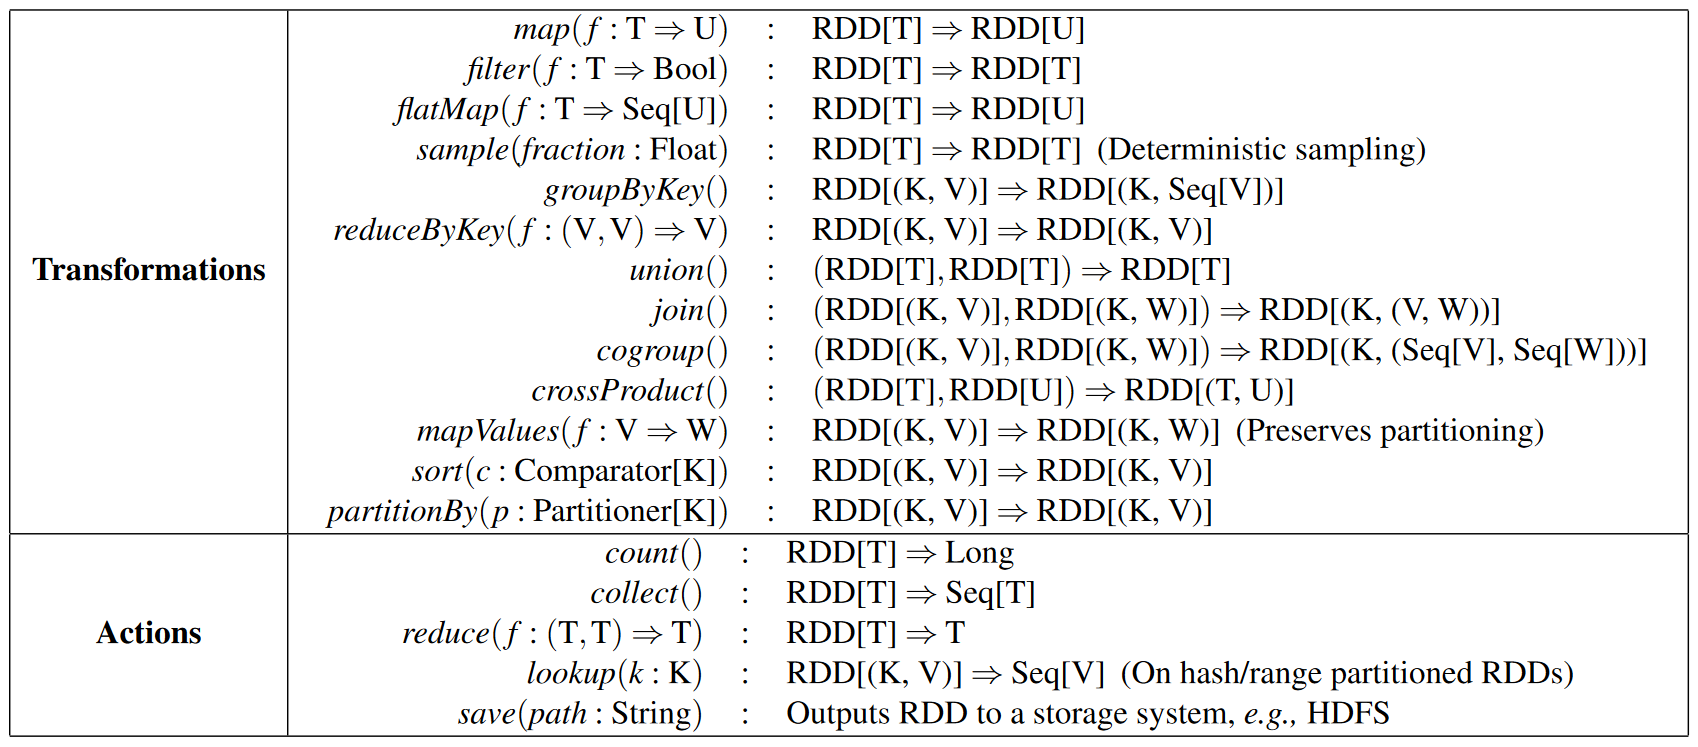
\includegraphics[width=1.0\textwidth]{images/spark-trans-action}
\label{Actions and Transformations}
\end{table}

\subsection{RDD fault-tolerance}

To begin the processing of an RDD, the individual data partitions (making up the source used to create the RDD -- typically a file in HDFS), are sent to different nodes in the computing cluster where the user defined DAC of operations is executed simultaneously for each partition (if the system could afford to allocate enough resources for a one-to-one mapping of partitions to cluster nodes). In a large scale distributed system, however, failure of individual hardware components is to be expected. When one of the cluster nodes fails, while processing an RDD partition, Spark is able to reconstruct the lost data without notifying the user.

Because RDDs provide an interface based on transformations (e.g., map, flatMap) that apply the same operations to many data items, they can efficiently provide fault-tolerance by logging the transformations used to build a dataset rather than the actual data (although checkpointing RDDs can have its advantages as previously mentioned). This log of operations is also known as the lineage of the RDD. Thus if a partition of an RDD is lost, the RDD has enough information about how it was derived from other RDDs to recompute just the missing partition\cite{RDD}. Therefore lost data can be quickly recovered without the need for costly replication.

The lineage of an RDD is a powerful property, since it ensures that a program cannot reference an RDD that it cannot reconstruct after failure -- it can always recompute all partitions from data in stable storage.

\subsection{RDD representation}

The Apache Spark framework provides a graph-based representation of RDDs where each dataset has a common interface, exposing five pieces of information:

\begin{itemize}
\renewcommand{\labelitemi}{\scriptsize$\blacksquare$}
\item a set of partitions, which are atomic pieces of the dataset
\item a set of dependencies on parent RDDs
\item a function for computing the dataset based on its parents
\item metadata about its partition scheme
\item metadata about its data placement
\end{itemize}

An RDD representing an HDFS file, for example, has as many partitions as the file has blocks and knows on which machine each block is located. If a map transformation were to be applied on this RDD, the resulting dataset would have the same partitions, but the map function would be applied on the parent's data when computing its elements.

An important aspect of this common interface is the representation of dependencies between RDDs. They are classified into two types: \textit{narrow} dependencies, where each partition of the parent RDD is used by at most one partition of the child RDD, and \textit{wide} dependencies where multiple child partitions may depend on a single parent partition\cite{RDD}. The \textit{map} operation would be an example of a narrow dependency, whereas \textit{groupByKey} would result in a wide dependency\footnote{Unless the RDD was explicitly hash partitioned beforehand.}.

The distinction between these two forms of dependencies has two primary implications. First, narrow dependencies allow for pipelined execution on one cluster node. This means that multiple successive operations resulting in narrow dependencies can be carried out on an RDD partition in the same computing cluster, without needing to move data between cluster nodes. Wide dependencies, however, require that data from all parent partitions to be available and to be shuffled across the nodes of the cluster. Second, narrow dependencies allow for a more efficient recovery from failure, as only the lost partitions need to be recomputed -- this can also be done in parallel on different processing nodes. When there are wide dependencies in the lineage graph of an RDD, however, a single failed node could loose information derived from all parent partitions, requiring a full re-execution of all transformations in the DAC, operating on the RDD.

\begin{figure}[H]
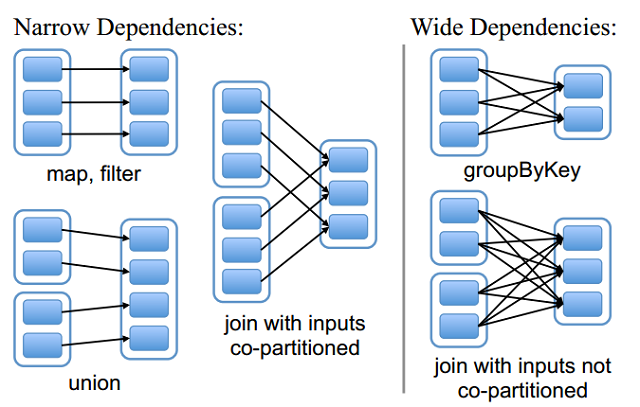
\includegraphics[width=1.0\textwidth]{images/rdd_dependency}
\caption{Examples  of  narrow  and  wide  dependencies.  Each box is an RDD, with partitions shown as shaded rectangles. (Source \cite{RDD})}
\label{RDD dependencies}
\end{figure}

\section{Shared Variables}

When invoking transformations on an RDD -- such as \textit{map} and \textit{filter}, developers pass closures (functions) to Spark. Similar to functional programming these closures can refer to any variable in the scope where they are created. Once Spark begins the execution of those transformations on a worker node, the referenced local variables are copied to the worker. However, Spark also allows programmers to create two restricted types of shared variables to support common usage patterns\cite{Spark}.

If a Spark program contains a large read-only piece of data that is used in multiple parallel operations, it is preferable to distribute it to the workers only once, as opposed to including it with each closure. This is accomplished by creating a ``broadcast variable'' object which acts as a wrapper for the desired value. It ensures that it is only copied once to each worker, thus reducing network traffic and improving performance.

Variables of the second type are known as ``accumulators''. Workers can only ``add'' to these variables by using an associative operation, and their value can only be read by the driver program. They enable easy implementations of counters (similar to MapReduce) and provide a more imperative syntax for parallel sums. Accumulators can be defined for any data type that has a ``zero value'' and an ``add'' operation.

\section{Spark Streaming}

In addition to its base API, Spark also provides a solution for developing applications based on scalable, high-throughput, fault-tolerant stream processing of live data. This is achieved thanks to Spark Streaming - a system that allows data to be ingested from many sources like Kafka, Flume, Kinesis, or TCP sockets, and later processed using complex algorithms expressed with high-level functions.

Once a Spark program defines an input data source, Spark Streaming can receive a live data stream from the specified source, which is then divided into batches that are later processed by the Spark engine. The primary abstraction that implements this operation is the \textit{discretized stream} or \textit{DStream}\cite{DStream}. It is represented internally as a sequence of RDDs.

Once a DStream has been created from a specified live data source (e.g., Kafka, an HDFS directory, whose content is being simultaneously altered by a different application, etc.) or alternatively from a different DStream, it begins to store or log any new information it has received. A program utilizing Spark Streaming needs to also specify a batch interval to the streaming context -- used to configure all DStreams for that application. At the end of every interval the DStream produces an RDD, containing all the data output from the specified source, since the start of the interval. The resulting RDDs are then processed by the remaining application logic -- various transformations and actions. Finally, the batch interval must be set based on the latency requirements of  the application and the available cluster resources.

\section{MLlib}

The Apache Spark project also includes a distributed machine learning library, built on top of Spark's core features -- MLlib. MLlib provides efficient functionality for a wide range of learning settings and includes several underlying statistical, optimization,
and linear algebra primitives. It exploits the benefits of Spark's fault-tolerant, parallel big data processing paradigm to deliver fast and scalable implementations of standard learning algorithms for common learning settings including:  classification, regression, collaborative filtering, clustering, and dimensionality reduction\cite{MLlib}.

MLlib also inter-operates well with Spark's other major components. Thanks to Spark SQL\cite{SQL} developers can more easily designate their prior storage solutions as the data source of the desired machine learning algorithms. Spark Streaming is also used by MLlib to enable applications to learn from real-time online streamed data, however, this is only supported by certain algorithms.

%==============================================================================

\chapter{K-Means Clustering}
\label{kmeans}

A long time pursuit in the field of artificial intelligence and machine learning has been to grant machines the ability to differentiate between discrete objects with similar or vastly different properties and to be able to identify and classify them. At a high level, an AI would need to be able to examine the features of an object, which has not been previously encountered and create an internal, digital representation of it. Then the machine would need to perform a computation on that model to extract meaning from it and predict the nature of the object, without human input - i.e., explicitly providing a label.

Recent developments in image processing and robotics have had a great impact on the field of machine learning, in regards to allowing systems that employ these practices to interact more directly in the real world. The aim of this paper, however, is not to cover techniques for creating a mapping from real world objects to internal, machine friendly representations of their properties, but rather to outline the implementation of algorithms for operating on said representations -- focusing on cluster analysis.

Cluster analysis is concerned with the task of grouping a set of objects in a way, such that objects in the same group (known as a cluster) are more similar to each other than those in other groups\cite{MLIntro}. It is commonly used in statistical data analysis as well as data mining. Along with machine learning, cluster analysis has applications in other fields such as pattern recognition, information retrieval, biometrics and others.

In cluster analysis, different approaches to the problem of grouping data together can vary greatly -- algorithms can differ in their notation regarding what constitutes a cluster, as well as how to find them. Popular definitions of clusters include: groups with small distances between the individual cluster members, dense areas of the data space or specific statistical distributions. Given a way of evaluating the quality of a particular assignment of individuals to groups, clustering can also be described as an optimization problem, were we are trying to maximize that value.

K-Means clustering is an examples of cluster analysis with a centroid-based model\cite{TopTen}. It was originally used in signal processing as a method for vector quantization. K-Means functions by partitioning \texttt{N} observable objects into \texttt{K} distinct clusters, where every object belongs to the cluster with the nearest mean  -- here these observations will only take the form of N-dimensional data points. The actual clusters are represented as a central vector (N-dimensional point), which does not necessarily belong to the input set.

\begin{figure}[H]
\centering
\begin{subfigure}{.5\textwidth}
  \centering
  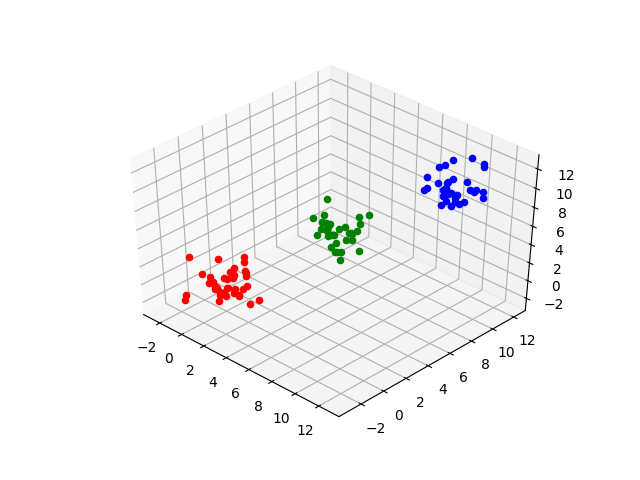
\includegraphics[width=1.2\linewidth]{images/figure_1}
  \label{fig:sub3}
\end{subfigure}%
\begin{subfigure}{.5\textwidth}
  \centering
  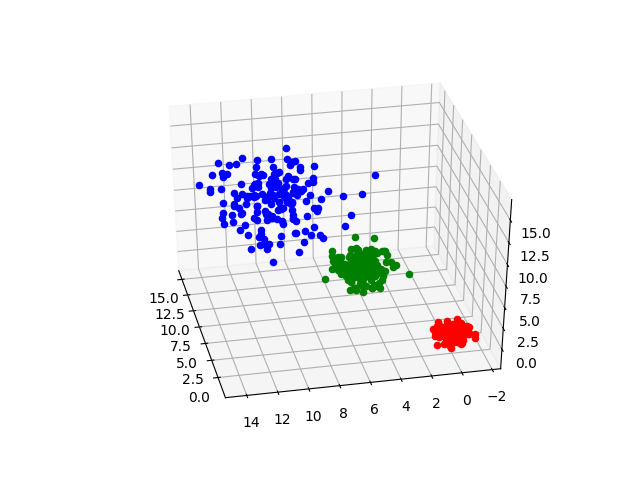
\includegraphics[width=1.2\linewidth]{images/figure_2}
  \label{fig:sub4}
\end{subfigure}
\caption{Examples of three distinct clusters in 3 dimensional space}
\label{basic clusters}
\end{figure}

When the number of centroids \texttt{K} is fixed, K-Means clustering provides a formal definition of an optimization problem: find the \texttt{K} cluster centers and assign the input data points to the nearest center, such that the sum of squared distances from the observed points to their respective centers is minimized. This is expressed by the Within-Cluster Sum of Squares (WCSS) formula:

\[ \scalebox{2}{$ arg_{s} min \sum_{i=1}^{k}\sum_{x \in S} \|x - \mu_{i} \|^{2} $} \]\\

Here $x_{1}$, $x_{2}$ ... $x_{n}$ is the set of observations in the form of multi-dimensional data points, $S_{1}$, $S_{2}$ .. $S_{k}$ are the \texttt{K} partitions of data points that are assigned to the \texttt{K} centers, and $\mu_{i}$ is the value of the centroid vector for partition $S_{i}$. This value is also referred to as the within-cluster sum of squares (WCSS) or the loss for the particular clustering\cite{MLIntro}.

The K-Means clustering optimization problem is also known to be NP-hard, therefore  a common approach is to simply search for approximate solutions. There is a number of efficient heuristic algorithms that quickly converge to a local optimum. Two of the most frequently used ones are Lloyd's algorithm (called Iterative K-Means here due to its reliance on iterative processing of the input data) and Mini-batch K-Means. These two algorithms will be examined in more detail as they present a proven method for deriving a practical result from a clustering operation and are already implemented as part of the API of MLlib.

Finally, it is worth considering that most forms of K-Means clustering require that the value of \texttt{K} is specified in advance. This is considered to be one of the main weaknesses of these algorithms as it is usually uncertain how many logical groups the data consists of. Similar issues with inconsistency can occur when poor initial values for the \texttt{K} centroids are chosen, as well as when the logical clusters, formed by the input data, are not approximately similar in size.

\section{Iterative K-Means Clustering}

Standard K-Means Clustering (Lloyd's algorithm), like all clustering algorithms examined here, is a form of unsupervised machine learning\cite{TopTen}. Its main  objective is to fit a set of cluster centers to the observed input data - both represented here as \textit{N}-dimensional data points. It achieves this through the use of an iterative refinement technique.

Given an initial set of \textit{K} means and a specified value of \textit{t} iterations, the algorithm proceeds to alternate between two main phases:

\begin{enumerate}
\item \textbf{Assignment}: Each observation is assigned to the center of a cluster, such that the within-cluster sum of squares (WCSS) is minimized. Because the sum of squares is the squared Euclidean distance, the assigned centroid is the ``closest'' one.
\item \textbf{Update}: Each centroid is updated to the value of the mean of all observations that were assigned to it. 
\end{enumerate}

These two phases are repeated \textit{t} times, providing a better heuristic answer after each iteration. Since the value of \textit{t} is defined prior to the start of the algorithm, it presents a clear quality for performance trade off. There is also a scenario where the values of the centroids will converge prior to the executions of all \textit{t} iterations. This is why most implementations of the algorithm include an optimization where if the values for the centroids are the same at the end of an iteration as they were at the star the algorithm will simply terminate. Another known optimization is to exploit triangular inequality to more efficiently compute the nearest centroid for each observed data point\cite{Triangle}. 

\begin{algorithm}
\caption{Iterative K-Means}\label{iterative}
\begin{algorithmic}[1]
\State Given: \textit{k}, iterations \textit{t}, collection of centroids \textit{C}, data set \textit{X}
\State Initialize each \textbf{c} $\in$ \textit{C} with an \textbf{x} picked randomly from \textit{X}
\For {i = 1 to t}
    \State v $\gets$ 0
    \State nextC $\gets$ 0
    \For {x $\in$ \textit{X}}
        \State \textbf{n} $\gets$ \textit{closestCenterIndex}(\textit{C},x) \hspace{0.4cm} // Get the index of the center nearest to \textbf{x}
        \State nextC[n] $\gets$ nextC[n] + x \hspace{1cm} // Add on the value of \textbf{x}
        \State v[n] $\gets$ v[n] + 1 \hspace{2.4cm} // Update per-center count
    \EndFor
    \State \textbf{end for}
    \For {\textit{c} $\in$ \textit{newC}}
        \State \textit{c} $\gets \frac{\textit{c}}{v[\textit{c}]}$ \hspace{1cm} // Average the value of the new centers
    \EndFor
    \State \textbf{end for}
    \State C $\gets$ newC \hspace{1.2cm} // Reasign the value of the centers
\EndFor
\State \textbf{end for}
\end{algorithmic}
\end{algorithm}

The fact that this algorithm needs to consider the whole set of data points multiple times limits its uses in regards to the quantity of data a user is willing to store. However, its execution does make it suitable for standard big data batch operations -- with the need to store and reload the data on every iteration being a major performance hindrance when using MapReduce.

\section{Mini-batch K-Means Clustering}

Mini-Batch K-Means clustering\cite{Mini} aims to resolve the scalability issue with standard K-Means in regards to storing all of the observed data and to provide low computation costs for working on large data sets -- capable of meeting the latency requirements of user facing applications.

It functions by taking small sample chunks of data form a source (mini-batches) and processing them one at a time. These mini-batches can be randomly sampled from a stored collection of data or they could be the output of a live data stream where each chunk needs to only be processed once without the need to store previous chunks.

Given an initial set of \textit{k} means and a considered mini-batch \textit{M}, the algorithm assigns each observed data point to one of the \textit{k} centers. For each point the weight of the closest center is increased by one and the center is updated according to the formula: $center = (1 - learningRate)center + learningRate * observedPoint$ where the learning rate is equal to $\frac{1}{clusterWeight}$.

\begin{algorithm}
\caption{Mini-batch K-Means}\label{mini-batch}
\begin{algorithmic}[1]
\State Given: \textit{k}, mini-batch size \textit{b}, iterations \textit{t}, collection of centroids \textit{C}, data set \textit{X}
\State Initialize each \textbf{c} $\in$ \textit{C} with an \textbf{x} picked randomly from \textit{X}
\State v $\gets$ 0
\For{\textit{i} = 1 to \textit{t} }
    \State \textit{M} $\gets$ \textit{b} examples picked randomly from \textit{X} 
    \For {x $\in$ \textit{M}}
    	\State \textbf{d}[x] $\gets$ \textit{f}(\textit{C}, x) \hspace{1cm} // Cache the center nearest to \textbf{x}
    \EndFor
    \State \textbf{end for}
    \For {x $\in$ \textit{M}}
    	\State \textbf{c} $\gets$ \textbf{d}[x] \hspace{1.5cm} // Get cached center for this \textbf{x}
        \State \textbf{v}[\textbf{c}] $\gets$ \textbf{v}[\textbf{c}] + 1 \hspace{0.5cm} // Update per-center counts
        \State $\mu \gets \frac{1}{\textbf{v}[\textbf{c}]}$ \hspace{1.5cm} // Get per-center learning rate
        \State \textbf{c} $\gets (1 - \mu)$\textbf{c} + $\mu$\textbf{x} \hspace{1cm} //Take gradient step
   \EndFor
   \State \textbf{end for}
\EndFor
\State \textbf{end for}
\end{algorithmic}
\end{algorithm}

This algorithm aims to provide an equal contribution, in regards to forming the centroids, for each observed point. However, because the data source could be a live stream where the centers of the logically formed clusters change more substantially over time, there is a proposed alteration to the algorithm where older observations have a smaller, decaying impact on the locations of the centers in comparison to newer observations\cite{Non-Stationary}. This can be achieved by changing the learning rate to a constant in the range $(0,1)$.

%==============================================================================

\chapter{Previous Work in MLlib}
\label{previous}

Iterative (Standard) K-Means and Mini-batch K-Means are two of the clustering algorithms already available through the machine learning library (MLlib) of Apache Spark. To better discuss the design decisions taken when implementing the proposed extension to MLlib, this paper will cover the approach taken by the previous Spark developers, for creating scalable versions of the K-Means Clustering algorithms. The considered version of Spark is 2.1.0.

\section{Implementation of Iterative K-Means Clustering}

Standard K-Means was the first clustering algorithm supported by Spark. Along with providing a useful machine learning utility, due to its reliance on iteration, standard K-Means was used as an example to showcase the benefits of Spark's in-memory processing for iterative batch jobs, versus the popular Hadoop MapReduce framework. Results showed that in this use-case Spark was able to offer more than a 2X improvement\cite{Comparison}.

\subsection{API details}

In the RDD based implementation of standard K-Means, MLlib exposes only a few functions the user needs to interact with the system. Primarily this is the \texttt{train()} method. While this is an overloaded method with many implementations it generally accepts all the input parameters needed to run the standard K-Means algorithm:

\begin{itemize}
\item \texttt{data}: An RDD holding all observed data points -- each being represented by a vector
\item \texttt{K}: The number of desired cluster centers
\item \texttt{maxIterations}: The maximum number of passes on the input data the algorithm will perform
\item \texttt{initializationMode}: A flag that determines the way the algorithm will select the initial value of the cluster centers
\item \texttt{seed}: A variable used to seed random functions used by the algorithm
\end{itemize}

The return value of this method (the result of running the algorithm) is a \texttt{KMeansModel} object. The representation of this object is an array with \texttt{K} vectors, each holding the value of a cluster center. It is important to note that that the output of a clustering job is not a mapping from input points to which center they belong to, but rather simply the values of the specified \texttt{K} centers. In order to obtain a mapping, a user would need to run a subsequent job, using the \texttt{KMeansModel} object to create a collection of key -- value pairs.

The \texttt{KMeansModel} object also includes the \texttt{computeCost()} method which calculates the loss of a model (i.e., the Within-Cluster Sum of Squares), given a set of input data points. This can be performed on any collection of data points as a measurement of how suitable the model is for the particular dataset, however, it is usually ran with the same RDD of vectors used to train the model.

Due to the fact that most clustering algorithms are merely trying to generate a set of centroids to fit against observed data points and that the WCSS is a reasonable performance measure for these algorithms the \texttt{KMeansModel} object is used as the output of all K-Means jobs.

\subsection{Algorithm details}

The operation performed by the \texttt{train()} method is to create an instance of the \texttt{KMeans} object (holding the implementation of the actual algorithm), to set the values of all provided parameters and to call the \texttt{run()} method. The \texttt{run()} method in turn is used only to transform the input data. 

The provided information consisting of N-dimensional points are represented as \texttt{DenseVectors}\footnote{A \texttt{DenseVector} is a collection where the value of every dimension of the vector is represented by a \texttt{Double}. In contrast a \texttt{SparseVector} does not include information of dimensions with a value of zero and is therefore represented by a mapping from indices to values for every non-zero dimension.} in MLlib. However, this algorithms also aims to make use of the triangle inequality, to gain better performance when computing the nearest centroid to a given point\cite{Triangle}. To achieve this, the \texttt{run()} method computes the Euclidean norm for each point and zips the two collections together to form an RDD of \texttt{VectorWithNorm} objects.

Finally the RDD of \texttt{VectorWithNorm} objects is passed to the \texttt{runAlgorithm()} method. Here the \texttt{initializationMode} flag is inspected to determine how the initial values of the \texttt{K} centroids will be set. One options is to have random initialization -- in this case the RDD of observed data points will be randomly sampled with the use of the \texttt{seed} parameter. The \texttt{K} extracted points will be used to set the starting values of the centroids. 

Alternatively, the centroids could be initialized by running the K-Means++ algorithm\cite{PlusPlus}. When K-Means++ is ran on a given dataset, it tries to find dissimilar cluster centers -- it starts with a random center and then performs passes where more centers are chosen with a proportional probability to the squared distance to their current cluster set. This method is far more expensive than the random initialization as it involves effectively running two separate algorithms on the data one after another. However, it is more likely that the final result will be of greater quality as it is likely to avoid some of the pitfalls related to poor centroid initialization. One way to mitigate this issue would be to run the K-Means++ algorithms on a small sample of the observed data, with a similar distribution, although the current API does not provide this option.

Once the values of the centroid vectors have been set, the algorithm begins its first of \texttt{maxIterations} passes on the data (the loop is also terminated if the centroids converge -- i.e., when an iteration of the algorithm has no effect on the location of the \texttt{K} centers). At the star of the iteration, broadcast variables for the current values of the centroids and a cost accumulator (used for logging) are created, so that they can be more efficiently used by different processing nodes. The rest of the algorithm is implemented by partitioning the set of input points and mapping an identical sequential operation across all the created partitions. 

At each cluster node, operating on a partition of the RDD of \texttt{VectorWithNorm} objects, the value of the centroids is retrieved from the previously created broadcast variable. Two blank arrays with a size equal to \texttt{K} are also created -- an array of sums for adding the values of observed point that ``attach'' to a particular centroid, and an array of weights for tracking how many points have ``attached'' to each centroid. Then, for each point in the partition, the closest centroid to that point is computed. The \texttt{findClosest()} helper method takes the processed point and array of center values and returns the index of the closest center in the array along with the distance to it. This is the method that required the input data to be converted to \texttt{VectorWithNorm} objects so that it can  make use of the triangle inequality optimization to compute the closest center faster\cite{Triangle}. After the index of the nearest centroid has been retrieved, the value of the weights array at that index is incremented, the values of each dimension of the considered point are added to the dimensions of the \texttt{Vector} object at the same index of the sums array and the distance between the centroid and the point is added to the accumulator.

Once all of the points have been processed, each partition outputs a collection of tuples with the following three values: the index of a centroid, the value that was accumulated at the same index in the sums array of that partition and the number of points that were added up to create the value in the sums array (i.e., the value of the weights array at that index for the same partition). The first value of the tuple (the centroid index) is then used as a key to group the outputs of the different partitions -- all tuples with an identical first element create one tuple where its second and third elements are the result of summing those elements across all relevant tuples.

Finally, the cluster centroids are updated by changing the value of each centroid at a particular index to the second element, divided by the third element of the tuple with a key (first element) equal to the index of that centroid. When reassigning each cluster center, the algorithm checks if the new value of the center is nearly equivalent to its previous value\footnote{The algorithm checks to see if the distance between the new and old value of the centroid is less than $\epsilon^2$, where $\epsilon$ is a predefined value.}.  If this is the case for all cluster centers then the algorithm considers that the result has converged and terminates, even if not all user specified iterations over the data have been executed. The function's output is a \texttt{KMeansModel} object, as discussed previously, generated from the final array of cluster centers.

\section{Implementation of Mini-batch K-Means Clustering}

Mini-batch K-Means or Streaming K-Means (as called in MLlib) aims to overcome the limitations of Standard K-Means in regards to storage, and provides the means to do real time data processing on live sources. It is an algorithm of particular interest, as its implementation is not only reliant on the core RDD based API of Spark, but it also utilizes Spark Streaming.

Because Mini-batch K-Means does not function by performing multiple passes on the entirety of the data, it is only required that one mini-batch from the whole data is available when the new value of the cluster centers is computed for each iteration. This relieves the user from having to store the entirety of available data to execute the algorithm. The notion that only a small chunk of the data is needed at any one time can be further abstracted to the idea that the entirety of the data has not even been created yet, and that the latest acquired piece is simply a partial output of a live data producing source.

For this reason Mini-batch K-Means was seen as a good example for implementing a machine learning algorithm that trains using real time data, obtained through Spark Streaming. A Spark application would monitor a stream (with data formated as N-dimensional data points) and between a specified time interval, collect all of the newly arrived points and process them as a single mini-batch.

\subsection{API details}

As was the case with Iterative K-Means the user exposed API of Streaming K-Means is fairly simple, however, there are several notable differences that arise from the use of streams. Firstly, as opposed to simply calling a \texttt{train()} method and receiving a \texttt{KMeansModel} object, one needs to instantiate a \texttt{StreamingKMeans} object and then call a series of mutator methods to provide the input parameters to the algorithm and establish the initial state of the \texttt{K} centroids. These methods include:

\begin{itemize}
\item \texttt{setK()}: sets the number of cluster centers
\item \texttt{setDecayFactor()}: sets the forgetfulness of centroids
\item \texttt{setHalfLife()}: sets the decay factor of centroids to $\exp(log(0.5) / halflife)$
\item \texttt{setInitialCenters()}: allows the user to manually enter the initial values for the \texttt{K} centers along with their staring weights - good to use if there are strong indications of what the data distribution will be like or if the user has a previously trained model that they would like to place in a streaming environment
\item \texttt{setRandomCenters()}: allows the user to specify the dimensions of the \texttt{K} centers, along with their starting weights and a seed. These parameters will be used to assign random initial centroids
\end{itemize}

The two alternatives for assigning the initial values of the \texttt{K} centroids are of particular interest. In contrast with the implementation for standard K-Means there is no option to set the initial values of the centroids to randomly selected points from the input set, or to run any centroid selection algorithm. This could be because the developers assume that the data available in the first encountered mini-batch could be either too small or unrepresentative of the expected distribution of points as time progresses. In fact the option to set a large starting weight for the initial centroids can be used to mitigate the effect of poorly distributed initial mini-batches.

Once all initialization has been completed, the algorithm can start executing by calling the \texttt{trainOn()} method and supplying an input discretized stream (\texttt{DStream}) of \texttt{Vector} objects. This method's implementation is to simply call the centroid updating algorithm for every RDD (mini-batch) produced by the DStream. After a certain amount of time has passed, or the stream has for some reasuon terminated, a user can inspect the latest value of the \texttt{K} centroids by calling the \texttt{latestModel()} method. Thus the final output of the Streaming K-Means algorithm is a \texttt{StreamingKMeansModel} object -- similar to the \texttt{KMeansModel} returned by Iterative K-Means, however, here a user also has access to the final weights attached to each centroid.

\subsection{Algorithm details}

Streaming K-Means functions primarily by making periodic updates to its \texttt{model} variable. It is an object of type \texttt{StreamingKMeansModel} -- a child inheriting from \texttt{KMeansModel} that also includes an array of weights for each of the \texttt{K} centers, along with an \texttt{update()} method. The \texttt{update()} method is responsible for changing the values of the \texttt{model} variable by operating on a single mini-batch -- to achieve this the program makes a call to \texttt{update()} from the \texttt{trainOn()} method for each RDD obtained from the DStream.

The \texttt{update()} function, invoked with an RDD of \texttt{Vector} objects, begins by using the input data to create an RDD of tuples with the following form (\texttt{closestCenterIndex}, (\texttt{originalPoint}, \texttt{1})). It then defines a \texttt{mergeContribs} function which takes two tuples of the form (\texttt{Vector}, \texttt{Long}) and produces another tuple with elements equal to the sum of the respective elements in the input tuples. The \texttt{aggregateByKey()} transformation is then invoked on the RDD of tuples with a (\texttt{vectorOfZeroes}, \texttt{0}) tuple as a starting value for each aggregated group and the \texttt{mergeContibs} function as a combining operation. This in effect sums the value of all points ``attached'' to a particular centroid and counts how many there are. Before changing the values of the existing centroids, however, a discount is applied to the weights array, allowing the algorithm to diminish the impact of old observations.\\ \\

Using the produced array of \texttt{K} tuples, each centroid corresponding to a tuple is updated as follows:

\begin{center}
\begin{BVerbatim}
lambda = numberOfSummedPoints / currentCentroidWeight
contributionVector = contributionVector * lambda
currentCentroid = currentCentroid * (currentCentroidWeight - 1)
currentCentroid = currentCentroid + contibutionVector
\end{BVerbatim}
\end{center}

As a final step the algorithm computes whether the cluster center with smallest weight is dying -- i.e., its weight is more than $10^8$ time smaller than the weight of the largest cluster. If this is the case the largest cluster is split in two and the centroid of the smallest cluster is destroyed.

%==============================================================================

\chapter{Proposed Extension to Spark/MLlib}
\label{propose}

One of the main drawbacks of the Iterative (standard) K-Means algorithm is its reliance on  multiple passes over the entirety of observed data. It does this in an attempt to minimize the Within-Cluster Sum of Squares (WCSS) value -- i.e., the loss of the resulting model of \texttt{K} centroids, however, it is also prone to get stuck in local maximums. Therefore its execution has the potential to incur a massive performance overhead, while offering little in added quality.

This paper covers a variety of possible alternative \textit{Online} clustering algorithms that, through performing a single pass over the provided data, can produce models that sacrifice little in terms of quality, but offer a substantial boost in performance. Certain approaches can overcome additional limitations of Standard K-Means, such as having to manually select a value for \texttt{K} without knowing how many logical centers the data might contain. These algorithms will first be examined from a mathematical perspective.

\section{Online K-Means}

One of the most basic forms of clustering that rely on a single pass of the observed data is Lloyd's Online K-Means algorithm. As is the case with the previously discussed algorithms, Online K-Means is a competitive learning algorithm, where, for each point belonging to a given input set, the \texttt{K} centroids compete to have that point ``attach'' to them -- the winner being decided based on which centroid is closest at the time the point is being considered\cite{MLIntro}. All of this serves to reduce the WCSS value.

A distinct aspect of Online clustering algorithms that is exemplified by Lloyd's Online algorithm is how every observed point has an immediate impact on its closest centroid. In the previous case of Iterative K-Means, the closest center for each observed point is calculated without making adjustments to the locations of the centroids, which are later reassigned to the average of all observed points that belong to the cluster they define. Here, upon encountering an input point and calculating which cluster it should belong to, the centroid of that cluster is immediately moved in the direction of the observed point, before considering the next one.

The amount of change a ``winning'' centroid experiences when encountering a new point is determined by the learning rate -- often depicted as $\eta$. In the original version of Lloyd's algorithm, the learning rate is expressed as the reciprocal of the number of points that had previously ``attached'' to a given centroid -- the weight of that centroid. 

\begin{center}
\begin{BVerbatim}
newCenter = oldCenter + learningRate * (observedPoint - oldCenter)
\end{BVerbatim}
\end{center}

It is clear to see that with a learning rate of 0, the center value would not change at all, and with a learning rate of 1, the new value of the center is the same as the observed point (i.e., 100\% of the value of that center is learned from the most recent point). Therefore, because Lloyd defines learning rate as 1/\textit{centerWeight}, as our input stream of data continues, each new encountered point will have a smaller and smaller impact on its closest centroid.

A possible alternative is to set the learning rate to a constant in the range $(0,1)$. This approach allows the algorithm to gradually forget the effects of older observed points, which lets it adjust better to the most recently formed logical centers.

\begin{figure}[H]
	\centering
    \includegraphics[width=0.65\textwidth]{images/Graph1HD}
    \caption{The empty circles are the centers and the black circle is an observed point. Online K-Means moves the closest center towards the direction of ($x-c_i$) by a factor of $\eta$.} 
    \label{onlineGraph}
\end{figure}

It is also important to note that Online K-Means is quite sensitive to the initial values of the \texttt{K} centroids. Because of its method of operation, if the centroids were cerated with poor starting values (e.g., two of the centroids being fairly close to one another), the final result could differ based on the order in which the points were observed.

\begin{algorithm}
\caption{Online K-Means}\label{online-alg}
\begin{algorithmic}[1]
\State Given: \textit{k}, collection of centroids \textit{C}, data set \textit{X}
\State Initialize each \textbf{c} $\in$ \textit{C} with an \textbf{x} picked randomly from \textit{X}
\State Initialize counters $n_{1}, n_{2} ... n_{k}$ with a zero value
\For {\textit{x} $\in$ \textit{X}}
    \State \textit{i}  $\gets$ \textit{getClosestCenterIndex}(\textit{C},x)
    \State \textbf{z}  $\gets$ C[i] \hspace{2.25cm} // Get the closest center
    \State n[i] $\gets$ n[i] + 1 \hspace{1.3cm} // Update the number of point in this cluster
    \State \textbf{z} $\gets$ z + $\frac{1}{n[i]}$ $\times$ (x - z) \hspace{0.35cm} // Update the cluster center
\EndFor
\State \textbf{end for}
\end{algorithmic}
\end{algorithm}

\section{Adaptive Resonance Theory K-Means}

In all of the clustering algorithms looked at so far a user specified value of \texttt{K} needed to be provided, before processing the available data. An expensive operation to determine a suitable \texttt{K} would be to run such an algorithm multiple times with different values of \texttt{K} and compare the resulting WCSS values of output models. This method, however, is not entirely reliable as the algorithm's intent is to find logical groups within the data, where as the value of WCSS (the loss of the produced model) will keep decreasing as \texttt{K} increases, and there is no clear indicator for when to stop\cite{LearnK}.

An alternative approach would be to incrementally discover a suitable value for \texttt{K} -- i.e., start with a single centroid and add more as they are needed. The Adaptive Resonance Theory (ART) algorithm\cite{ART} is one such example. In the case of ART, instead of requiring a set value for how many centroids will be trained, the algorithm takes as input a threshold value called a \textit{vigilance} (specifying a Euclidean distance in this case). 

Thus ART K-Means begins by assigning a single centroid to have the same initial value as a point, randomly selected from the input set. Then, for each new processed point, the nearest available centroid is identified (there will be only one at the start). If the distance between the observation and its closest centroid is less than the specified vigilance, the respective cluster center will be updated in the same manner as Online K-Means (Algorithm \ref{online-alg}). If the distance is greater than the vigilance, however, a new centroid is created at the location of the examined point.

\begin{figure}[H]
	\centering
    \includegraphics[width=0.65\textwidth]{images/Graph2HD}
    \caption{The distance from $x^a$ to the closest center is less than the vigilance $\rho$ -- the center is updated in the same way as Online K-Means. $X^b$ is not close enough to any of the centers and so a new centroid should be created at its position.} 
    \label{artGraph}
\end{figure}

The \textit{vigilance} value used in ART K-Means effectively defines a hypersphere around each centroid. Therefore, any new point that does not fall within the boundaries of an existing hypersphere creates a new one. This results in the partitioning of the examined N-dimensional space and sets a clear boundary for the region occupied by any given cluster. 

\begin{algorithm}[H]
\caption{ART K-Means}\label{art-alg}
\begin{algorithmic}[1]
\State Given: vigilance value $\rho$, collection of centroids \textit{C}, data set \textit{X}
\State Initialize one \textbf{c} $\in$ \textit{C} with an \textbf{x} picked randomly from \textit{X}
\State Initialize a single counter $n_{1}$ with a value of zero
\For {\textit{x} $\in$ \textit{X}}
    \State \textit{i}  $\gets$ \textit{getclosestCenterIndex}(\textit{C},x)
    \State \textbf{z}  $\gets$ C[i] \hspace{2.35cm} // Get the closest center
    \State \textbf{d} $\gets$ \textit{getDistance(x, z)} \hspace{0.3cm} // Get the distance between the point and its nearest center
    \If {$d < \rho$}
        \State n[i] $\gets$ n[i] + 1 \hspace{1.3cm} // Update the number of point in this cluster
        \State \textbf{z} $\gets$ z + $\frac{1}{n[i]}$ $\times$ (x - z) \hspace{0.35cm} // Update the cluster center
    \Else
        \State \textit{C} $\gets$ \textit{C} + \textit{x} \hspace{0.55cm} // Create a new center with a value equal to the observed point
        \State $n_k$ $\gets$ 1 \hspace{1cm} // Create a counter for the new center with a weight of one
    \EndIf
\EndFor
\State \textbf{end for}
\end{algorithmic}
\end{algorithm}

ART K-Means does not entirely solve the issue of specifying an initial number of centroids but rather shifts the problem to choosing an optimal \textit{vigilance} value. Because it is possible to identify the extremes of any of the dimensions of the input points, however, one can adjust the vigilance to partition the observed space into a set number of equally sized hyperspheres. This overcomes a different weakness of traditional clustering algorithms, where the initial values of the \texttt{K} centroids could be insufficiently dissimilar (e.g., two centroids starting off at nearly identical coordinates).

\section{Self-Organizing Maps K-Means}

All of the competitive clustering algorithms looked at so far have taken a ``winner take all'' approach -- i.e., for every new observed point, only the centroid closest to it experiences change. However, in an online learning environment where the model needs to adapt to a constant stream of new data, that is likely to alter its distribution over time, it is possible to encounter ``dead'' centroids.

For example, consider at time $t_0$ Online K-Means is run on a continuous data source that provides a distribution with three logical groups. If the state of the model were to be probed at time $t_1$ then (assuming a suitable initialization) it would correctly consist of three centroids that identify the different groups. If at time $t_2$, however, the data source stopped producing output that belongs to one of the groups (the group has ``died'') and the state of the model were to be probed afterwards, it would continue to indicate that the data consists of three distinct clusters.

A way to avoid dead centers is to update not only the winner, but also a few additional centroids. In the Self-Organizing Map (SOM) each cluster center is assigned an index, which defines a neighborhood of centroids\cite{SOM} -- in this context also called neurons. When $c_i$ is the closest center to an observed point, the neighbors of $c_i$ are also moved. If the neighborhood is of size 2, then $c_{i-2}, c_{i-1}, c_i, c_{i+1}, c_{i+2}$ are all adjusted, but with less weight as the neighborhood increases.

In the case of SOM K-Means each neuron is updated with respect to ``the impact of the neighborhood''. It is defined as a Gaussian function of the Euclidean distance of the locations of the neurons in the neighborhood -- for two neighboring neurons \texttt{A} and \texttt{B} the impact is:  $h(A,B) = \exp(-\sigma \times distance(A, B)^2)$. Thus if $W^{\prime}$ is the closest center to an observed point \textit{X} then all neurons \textit{W} in the neighborhood are updated by the formula:

\begin{figure}[H]
\begin{CenteredBox}
  \begin{lstlisting}
    $W = W + h(W^{\prime},W)\times\eta\times(X-W)$
  \end{lstlisting}
\end{CenteredBox}
\end{figure}

It is clear to see that when it comes to updating the ``winning'' center itself, the impact function will evaluate to 1 (the distance between the winner and himself is 0) and the formula will become:

\begin{figure}[H]
\begin{CenteredBox}
  \begin{lstlisting}
    $W = W + \eta\times(X-W)$
  \end{lstlisting}
\end{CenteredBox}
\end{figure}

This is identical to the update step used in Lloyd's Online K-Means algorithms, as well as ART K-Means when the observed point falls within an existing hypersphere.

\begin{figure}[H]
	\centering
    \includegraphics[width=0.65\textwidth]{images/Graph3HD}
    \caption{In the SOM, the closest center and its neighbors (in terms of indices) are all moved towards the observed point. Here the neighborhood is of size 1 and the 1-nearest neighbors are updated. Even if the neighbors are not close to each other, as they continue to influence each others locations, they will also become neighbors in the input space.} 
    \label{somGraph}
\end{figure}

In SOM K-Means, because neighboring neurons are also moved towards the input, dead centroids are avoided, as they will eventually win a competition, after being consistently adjusted by the previous winners. This is highly desirable in an online learning environment, as the underlying model will consistently reflect the present state of the data distribution.

It is also important to consider that neighboring centroids by indices need not necessarily be physical neighbors in the input space. Typically, the starting value of each centroid will be randomly chosen and their proximity in indices will not reflect their Euclidean distance. As the model is trained, however, because the winning centroid and its neighbors are all influenced together by the same input, after the algorithm converges, centroids with neighboring indices will also be neighbors in the input space.

While this illustrates the operational model of SOM, most applications that utilize this approach introduce an additional layer of complexity by organizing the neurons in a two-dimensional map. In this scenario, each neuron has two indices (row and column) which represent its location on a 2-D lattice. Here, the neighborhood of a neuron is also defined in two dimensions -- a neighborhood of size one refers to all adjacent neurons in the lattice, while size two would refer to every neuron in a 5x5 lattice centered on the winner (every neuron reachable by two or less hops). If the winning centroid happens to be a member of the left most column, its left side neighbors are the members of the right most column of the lattice -- it functions as a torus.

\begin{figure}[H]
	\centering
    \includegraphics[width=0.5\textwidth]{images/latticeHD}
    \caption{A 5x5 SOM lattice of neurons with a neighborhood of size one. Here the central neuron is closest to the observation. This updates its value along with all of its neighbors.} 
    \label{somLattice}
\end{figure}

After the locations of the neurons have converged, the resulting 2-D lattice will represent a \textit{topological map} of the original N-dimensional input space. The map will contain several neurons in parts of the space where there was a high density of observations, and no neurons in places that didn't have any input data. Because of this, the map can be interpreted as doing a nonlinear form of multidimensional scaling, which maps from the original N-dimensional space to two dimensions\cite{MLIntro}. Furthermore, if the map is one-dimensional (as originally discussed), the neurons are placed on the curve of maximum density in the input space -- i.e., a \textit{principal curve}\cite{SOM}.

\begin{algorithm}[H]
\caption{SOM K-Means}\label{som-alg}
\begin{algorithmic}[1]
\State Given: dimension of neuron lattice \textit{M}, neighborhood size \textit{H}, tuning parameter $\sigma$
\State \hspace{1.1cm} learning rate $\eta$, collection of neurons \textit{C}, data set \textit{X}
\State Initialize each \textbf{c} $\in$ \textit{C} with an \textbf{x} picked randomly from \textit{X}
\For {\textit{x} $\in$ \textit{X}}
    \State \textit{i}  $\gets$ \textit{getclosestCenterIndex}(\textit{C},x)
    \State \textbf{z}  $\gets$ C[i] \hspace{3.85cm} // Get the winning neuron's index
    \State \textbf{z} $\gets$ z + $\eta \times$ (x - z) \hspace{2.35cm} // Update the winning neuron
    \State \textbf{N} $\gets$ getNeighborNeurons(C, H) \hspace{0.1cm} // Get all neurons in the neighborhood of the winner
    \For {n $\in$ N}
        \State \textit{d} $\gets$ getDistance(n, z) \hspace{1.3cm} // Calculate distance to the winner neuron
        \State \textit{impact} $\gets$ $\exp(\sigma \times d^2)$ \hspace{1.15cm} // Calculate the impact of the neighborhood
        \State \textbf{n} $\gets$ n + \textit{impact} $\times \eta \times$ (x - n) \hspace{0.3cm} // Update the neighboring neuron
    \EndFor
    \State \textbf{end for}
\EndFor
\State \textbf{end for}
\end{algorithmic}
\end{algorithm}

\section{Benefits of Online Algorithms}

Due to the present state of available information gathering and live data streaming technologies, real time processing of new information is becoming increasingly more desirable. As new data is constantly made available to a machine learning reliant application, its underlying model needs to continuously adapt in order to accurately reflect the present state of the world around it.

The above discussed clustering algorithms provide a means of performing online unsupervised learning from a data stream, resulting in a responsive underlying model. They overcome the performance overhead of iterative data processing, as well as the requirement to persist all observed information, which would quickly become infeasible in an online learning environment. Furthermore, the presented algorithms offer a variety of input parameters and underlying model adjustment schemes, allowing for greater user choice in regards to satisfying the particular needs of an application -- e.g., is there a particular way the input space should be partitioned between clusters, should dead centroids be avoided, etc. 

\section{Implementation Challenges in Parallelizing Online Clustering Algorithms}

When executing the Iterative or Mini-batch K-Means algorithm, the effect of every observed point (in the entire batch or mini-batch respectively) is aggregated before making an adjustment to the model of centroids. Thus, Spark implements these two algorithms by parallelizing the computation of each observations' impact and later making an update to the model in a local sequential process.

In contrast, online clustering algorithms perform an immediate update to the state of the centroid model for each new observation. Therefore, parallelizing the effect of observations taken from a high volume stream becomes a non-trivial task. If a collection of input vectors is distributed between multiple partitions, updates to the model in one partition are not visible to others, while the most recent state of the model is constantly required to decide which centroid will be the ``winner'' regarding the latest data item.

To overcome this issue it is necessary to employ additional data partitioning techniques along with a variety of partial solution combination algorithms. These methods can result in marginally reducing the quality of the final result, however, they are necessary to enable the performance benefits obtained from Spark's parallel data processing model.

%==============================================================================

\chapter{Online K-Means}
\label{online}

Two alternative implementations of Online K-Means were created -- one that functions as a single large batch process and another that relies on the facilities of Spark Streaming. The two designs also take alternative approaches in their data partitioning and solution combination phases.

\section{Implementation Using Grand Mean}

The first created implementation of the Online K-Means Clustering algorithm emulates the approach taken by Spark's previous developers in creating the standard iterative algorithm. The program is once again structured as a discrete batch operation, relying on Spark's RDD API.

\subsection{API details}

The implemented class exposes only a single public method: \texttt{train()} which is necessary to execute the algorithm. It takes the following input parameters:

\begin{itemize}
\item \texttt{data}: An RDD holding all observed data points -- each being represented by a vector
\item \texttt{K}: The number of desired cluster centers
\item \texttt{seed}: A variable used to seed the sampling, necessary to make the initial centroid selection
\end{itemize}

The return value of the \texttt{train()} method is once again a  \texttt{KMeansModel} object, holding an array with \texttt{K} vectors, each representing the final location of a computed cluster center. In order to obtain the resulting WCSS value, one can simply invoke the model's \texttt{computeCost()} method and provide the same RDD of vector data as an input parameter.

\subsection{Algorithm details}

The underlying functionality of the \texttt{train()} method is to simply create an instance of the \texttt{OnlineKMeans} object, passing on the previously mentioned parameters, and invoke the object's \texttt{run()} method. As was the case with the implementation of standard K-Means, the \texttt{run()} method's function is to transform the input data into \texttt{VectorWithNorm} objects, thus enabling the use of the triangle inequality optimization for obtaining better performance when computing the nearest centroid to a given point\cite{Triangle}. Finally, the \texttt{run()} method returns a centroid model by invoking the \texttt{runAlgorithm()} function on the RDD of \texttt{VectorWithNorm} objects.

The \texttt{runAlgorithm()} function in turn parses the transformed RDD and computes the resulting centroids. It begins by using the \texttt{seed} parameter to randomly sample the RDD and extract \texttt{K} vectors, which are used as the initial locations of the cluster centers. Then a broadcast variable holding the value of the \texttt{K} centroids is created (in order to reduce network traffic) and the \texttt{mapPartitions()} transformation is invoked on the RDD. This transformation is used to map an identical sequential operation across every partition of the RDD stored on different processing nodes. In the present scenario, the sequential operation is an implementation of the Online clustering algorithm (alg. \ref{online-alg}).

This step is of particular interest as it can result in greatly influencing the final result of the function. Because no additional effort has been made to manually enforce a partitioning scheme on the data, the default partitioning of the provided RDD of vectors is used. If the data held in different partitions of the RDD does not have a uniform distribution across all logical clusters, there could be a large skew in the final output of the algorithm -- e.g., data consists of 3 logical clusters and 2 partitions -- partition 1 holds all observations from 2 of the clusters, partition 2 holds all data from the last cluster.

\begin{figure}[H]
	\centering
    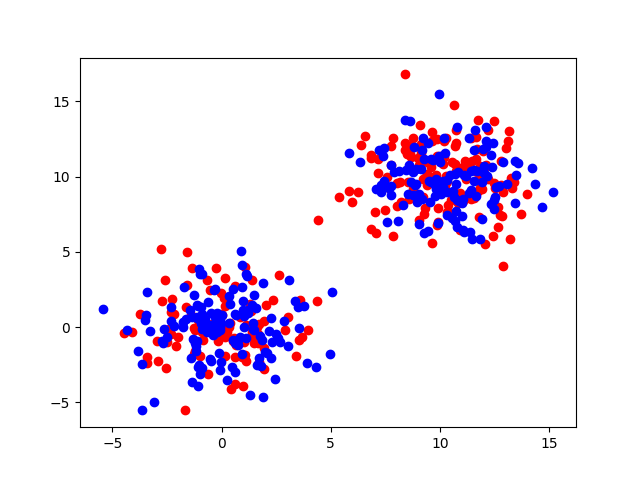
\includegraphics[width=1.0\textwidth]{images/partitions}
    \caption{An example partitioning of 2 dimensional input data points. Every blue point belongs to the first partition, every red one to the second.} 
    \label{partitions}
\end{figure}

The first operation performed in the \texttt{mapPartitions()} transformation is to inspect the value of the broadcast variable holding the initial locations of the \texttt{K} centroids and create a deep copy of it. Because each individual processing node will be making updates to the values of the centroids, they need to have their own unique copies, so as to not overwrite each other's results. An array of weights, holding the number of vectors that have ``attached'' to any given centroid, is also created.

For each point, present in a given partition, the closest centroid (in terms of Euclidean distance) is identified, making use of the triangle inequality optimization, and the weight of that centroid is incremented. Immediately after, the value of the centroid is updated in the following way:

\begin{center}
\begin{BVerbatim}
newCenter = oldCenter + learningRate * (observedPoint - oldCenter)
\end{BVerbatim}
\end{center}

Here the learning rate is expressed as the reciprocal of the weight of the centroid, meaning that each new observation has a smaller and smaller impact on the location of the cluster center. Furthermore, since the coordinates of the centroid have shifted, it is necessary to recompute the vector's euclidean norm, so that subsequent input vectors can correctly identify their closest centroid. 

Once all observations have been processed, every partition outputs a collection of tuples, each holding the coordinates of one of the \texttt{K} centroids along with its weight. Therefore, if the original RDD of vectors held \texttt{N} partitions, \texttt{N} $\times$ \texttt{K} tuples would be obtained. These resulting tuples present each partition's incomplete solution to the clustering problem (due to operating on a subset of the data).

As a final step, it is necessary to combine the \texttt{N} $\times$ \texttt{K} tuples of partial solutions in order to obtain the final result. This is achieved by aggregating groups of \texttt{N} tuples into one centroid. For each center coordinate that has not yet been considered, the closest (by euclidean distance) \texttt{N} - 1 centers are identified and then merged based on a weighted average. The produced \texttt{K} vectors are then used to instantiate a \texttt{KMeansModel} object, which is returned to the user.

\begin{algorithm}[H]
\caption{Computing the grand mean of partial solutions of Online K-Means}\label{online-merge}
\begin{algorithmic}[1]
\State Given: \textit{N} $\times$ \textit{K} tuples of (centerCoordinate, centerWeight) $\in$ \textit{T}, an empty results set $T''$ 
\For {\textit{t} $\in$ \textit{T}}
    \State \textit{T}  $\gets$ \textit{sortByDistanceTo}(\textit{t})
    \State $T'$ $\gets$ T.takeFirst(\textit{N})
    \State $t'' = ([0 ,0, .., 0], 0)$
    \For {$t' \in T'$}
    	\State totalWeight $\gets$ $t''$.weight + $t'$.weight
        \State $t''$.center $\gets$ ($t''$.weight/totalWeight) $\times t''$.center
        \State $t'$.center $\gets$ ($t'$.weight/totalWeight) $\times t'$.center
        \State $t''$.center $\gets$ $t''$.center + $t'$.center
        \State $t''$.weight $\gets$ totalWeight
    \EndFor
    \State \textbf{end for}
    \State $T'' \gets T'' + t''$
    \State \textit{T} $\gets$ \textit{T}.removeAll($T'$)
\EndFor
\State \textbf{end for}
\end{algorithmic}
\end{algorithm}

Originally, the partial solution combination phase was implemented by tracking each centroid's index (in the array of centroids that is copied over by each partition) and performing a weighted average over centroids with an identical index. This proved inadequate, however, as there is the possibility that centroids with an identical starting location could ``attach'' themselves to different clusters of the data in different partitions. Thus averaging them based on their indices could create a final centroid, situated between two clusters.

\section{Implementation Using Spark Streaming}

While the previous implementation of Online K-Means demonstrates a means of computing cluster centers by performing a single pass over the RDD of observations, it has a major weakness -- the user is expected to store all of the clustering data  prior to running the algorithm. This would make the Grand Mean implementation impractical for the purposes of constructing an application, relying on continuous online learning from live sources. 

To overcome this downside, another version of the Online K-Means algorithm was created, which makes use of the facilities provided by Spark Streaming. In a similar fashion to the previous implementation, the new design emulates the approach taken by Spark's previous developers in creating the \texttt{StramingKMeans} class.

\subsection{API details}

To launch the Online K-Means algorithms, with a stream of N-dimensional vectors as a data source, it is first necessary to instantiate a \texttt{StreamingOnlineKMeans} object. Then, one has to invoke a series of mutator methods to provide all the required input parameters to the program and possibly establish an initial state for the \texttt{K} centroids. The methods include:

\begin{itemize}
\item \texttt{setK()}: sets the number of cluster centers
\item \texttt{setSeed()}: set a seed for the random sampling, used to make an initial centroid selection
\item \texttt{setInitialCenters()}: allow the user to manually set the starting values of the \texttt{K} centroids, along with their initial weights -- especially useful if the rough locations of the clusters are already known, or if a developer has a previously trained model, which they would like to place in a streaming environment 
\end{itemize}

After all the necessary initialization has been completed, the algorithm can begin executing by calling the \texttt{trainOn()} method and providing as input a discretized stream (DStream) of Vector objects -- this will become the monitored continuous data source. For every produced RDD, the method will make a call to the centroid updating algorithm, which will process the effect of all new observations. 

Furthermore, once the first RDD is retrieved from the DStream, the supplied \texttt{seed} parameter is used to sample its contents and retrieve \texttt{K} random vectors, which will be used as the starting locations of the \texttt{K} centroids. This implementation can prove problematic, however, as the first retrieved RDD might hold observations which are not representative of the long term distribution of data. In an attempt to amend this issue, the \texttt{setInitialCenters()} method is provided which, if invoked prior to training the model, will circumvent the random initialization of centroids.

Finally, after enough batch intervals (defined by the Streaming Context) have passed and a suitable quantity of data has gone through the system, the present values of the \texttt{K} centroids can be inspected by calling the \texttt{latestModel()} method. Its return value is a \texttt{StreamingOnlineKMeansModel} object, which is a child of the typically used \texttt{KMeansModel}, but it also holds the weights of each centroid and provides the implementation of the \texttt{update()} method.

\subsection{Algorithm details}

Similarly to the existing Streaming K-Means program in MLlib, the presented implementation of the Online K-Means algorithm functions by performing periodic updates to a \texttt{model} variable. It is an object of type \texttt{StreamingOnlineKMeansModel} which holds the centroid coordinates, their weights and an \texttt{update()} method. In order to keep the model relevant, the \texttt{trainOn()} method makes a call to \texttt{update()} for each RDD produced by the DStream -- supplying said RDD as an input parameter.

The \texttt{update()} function, having received an RDD of \texttt{Vector} objects, proceeds to create an RDD of tuples where the second element is an observed point and the first is the nearest current centroid to that point (since this operation does not affect the state of the model it is trivial to parallelize with \texttt{map()} transformation). After broadcast variables for the arrays holding the coordinates of the cluster centers and their weights are created, the RDD of tuples undergoes the \texttt{groupByKey()} and \texttt{mapPartitions()} transformations. These two operations are of particular interest as they dictate how the observations will be used to update the model.

The \texttt{groupByKey()} operation is used to used to alter the underlying structure of an RDD from a collection of key-value pairs (split between different partitions) to objects of the form -- (key, Iterable(value)), where one or more of these objects are stored in a single partition. This means that all points that are likely to influence a particular centroid are guaranteed to be present in a single partition. Being a transformation with wide dependencies\footnote{A transformation with wide dependencies needs to shuffle data between partitions, generating additional overhead and network traffic. In contrast a transformation with narrow dependencies does not need to move data between partitions.}, calling \texttt{groupByKey()} is fairly expensive, however, it has two major upsides:

\begin{enumerate}
\item Because the algorithm utilizes Spark Streaming, the \texttt{groupByKey()} transformation will be applied to an RDD produced by a DStream, which is expected to hold a relatively small number of observations, resulting in a far less severe performance impact.
\item Due to the fact that no two partitions will hold points that will influence the location of the same centroid, the execution of the Online K-Means algorithm can be parallelized across multiple worker nodes, without having to combine the partial solutions of each worker with a weighted average at the end. This eliminates the possibility of having the final results being skewed by a poor default partitioning of the input vectors across processing nodes. 
\end{enumerate}

\begin{figure}[H]
	\centering
    \includegraphics[width=0.65\textwidth]{images/partitions2HD}
    \caption{An example partitioning of input data points based on their proximity to existing centroids -- the white circles are centroids, the black ones are new observations.} 
    \label{partitions2}
\end{figure}

As part of the operation performed on each partition, deep copies of the arrays of centroid locations and their weights are obtained from the values of the previously created broadcast variables. Then, all groups of vectors that have attached themselves to an existing centroid, sent to the current partition, are processed sequentially.

For each group of data points, the respective centroid and its weight are retrieved. The effect of each observation on the center's location is then computed through the standard formula:

\begin{center}
\begin{BVerbatim}
newCenter = oldCenter + learningRate * (observedPoint - oldCenter)
\end{BVerbatim}
\end{center}

The learning rate is once more expressed as the reciprocal of the weight of the centroid, which is incremented for each new observation. Unlike the previous implementation of the Online K-Means algorithm, since the centroid that each point will influence has already been determined, it is not necessary to recompute the euclidean norm of the centroid after each update.

Before terminating its execution, every worker node, operating on a separate partition, outputs a collection of (center index, (center coordinates, weight)) tuples, for each centroid that had its new values recomputed at that node. Therefore, since every centroid is updated by only one node, there are no two tuples referring to the same centroid. In this case, it is simply enough to overwrite the coordinate and weight values in the appropriate arrays at the indicated centroid indices. It is important to note that the old arrays are not simply replaced by the aggregation of the output tuples, as there could have been centroids, that received no update from the data found in the latest RDD and so they would not have a corresponding output tuple.

Once this operation has completed, the changes to the model, brought about by the input RDD of vectors, have been applied and the system enters a consistent state with a single view of the \texttt{K} centroid coordinates. Now the program is ready and waiting for the DStram to output another RDD so that this process may begin again.

Had this approach been implemented without Spark Streaming, the input data partitioning scheme currently used would have resulted in exceptionally poor results. In fact, because the centroid that would be influenced by an observation is determined before any update to the model, the result would have been equivalent to performing a single iteration of the standard K-Means algorithms. With streaming, however, the program makes small periodic updates to its model, which alter the way in which input vectors with an identical distribution are partitioned between the centroids, for each consecutive RDD.\\\\

\begin{figure}[H]
	\centering
    \includegraphics[width=1.0\textwidth]{images/DStream}
    \caption{An illustration of consecutive updates to the \texttt{K} centroids, caused by processing in parallel the data held in each RDD, produced by a DStream.}
    \label{DStream}
\end{figure}

%==============================================================================

\chapter{Adaptive Resonance Theory K-Means}
\label{art}

While the previously discussed implementations for Online K-Means present a way to achieve highly efficient and scalable clustering in an online learning environment, they have a number of weaknesses, stemming from the nature of the underlying algorithm. These shortcomings exists primarily because of the users potential uncertainty about the distribution of available data, as well as the possibly poor selection of the \texttt{K} centroids' initial coordinates.

When operating with a continuous live source of data, or any vast quantity of information that did not originate from the observation of a discrete number of entities, it is often the case that the number of logical groups that exist amongst the gathered samples will be unknown. The algorithms, whose implementation has been looked at so far, however, all require the user to specify the value of \texttt{K} prior to processing the data. Furthermore, the method of setting the initial values of the \texttt{K} centroids, through randomly sampling the input data, can result in highly inaccurate clustering results if a significantly large percentage of the centroids are  initialized with nearly identical coordinates\cite{PlusPlus}.

The purpose of developing ART K-Means with the use of Spark Streaming is to take advantage of the benefits offered by the Online K-Means algorithm (not having to iteratively process all observations, not needing to store the entirety of the data, etc.) while simultaneously overcoming its potential weaknesses. This is all achieved by reducing the users responsibility, in regards to specifying the exact number of desired centroids.

\section{Alterations to the Adaptive Resonance Theory Algorithm}

In the Adaptive Resonance Theory algorithm, the final value of \texttt{K} is incrementally discovered while processing the data -- the algorithm begins with a single centroid and adds more when it is necessary. Whether a new observation will influence an existing cluster center or will require the creation of a new one is determined by a user specified value, known as the \textit{vigilance} (normally expressed as an euclidean distance). If the distance from the latest observation to its closest centroid is less than the \textit{vigilance} value, the centroid coordinates are adjusted according to the standard online clustering formula:

$$W' = W' + \eta(X - W')$$

\noindent where $W'$ is the ``winning'' centroid, $X$ is the latest observation and $\eta$ is the learning rate. If the distance form $W'$ to $X$ is greater than the vigilance, however, a new centroid will be instantiated with the same coordinates as $X$. In this way, the algorithm effectively partitions the available N-dimensional space into a series of hyperspheres, with a radius equal to the \textit{vigilance} value.

While this technique in adequate when dealing with a low-dimensional setting, such as the 3D physical space, it becomes unintuitive for a user to supply a value specifying euclidean distance between points with hundreds or thousands of dimensions -- the Curse of Dimensionality\cite{CurseOfDimensionality}. To overcome this, it is necessary to provide the user with a different means of expressing the radius of the hypersphere surrounding each centroid.

The solution proposed by this paper involves normalizing the values of all centroids and observations, so that they fit within the confines of a unit hypercube -- i.e., transform the value of each dimension of a given point to fit between 0 an 1. This is achieved by defining two special vectors: \textit{max} and \textit{min}, where \textit{max} holds the maximum possible value for each dimension and \textit{min} tracks the minimum possible value of each dimensions. If normalized, the \textit{max} and \textit{min} vectors would become $[1, 1, 1, ..., 1, 1]$ and $[0, 0, 0, ..., 0, 0]$ respectively. Then, to normalize a vector $X$, for each dimension $i$ the following formula is applied:

$$X'[i] = \frac{X[i] - min[i]}{max[i] - min[i]}$$

It is important to note that, when working in normalized space, the maximum possible distance between any two points is the distance between the \textit{min} and \textit{max} vectors defined as:

$$\|max - min\| = \sqrt{(1-0)^2 + (1-0)^2 + ... + (1-0)^2} = \sqrt{numDimensions}$$

\noindent Therefore, the squared distance between the \textit{min} and \textit{max} vectors is also equal to the number of dimensions in the observed data. It is then clear that the squared distance between any two points in the unit hypercube is between 0 and the number of dimensions of the hypercube. 

For the purposes of the ART K-Means algorithms, one can now reasonably express the \textit{vigilance} value, as any number between 0 and the number of dimensions in the observed space. Then, the squared distance between the normalized forms of an observation and its closest centroid can be measured up against the \textit{vigilance} to determine if a new centroid should be created.

\section{API Details}

To run the ART K-Means algorithm, with a DStream of vectors as a live data source, it is first necessary to instantiate an \texttt{ARTK-Means} object. Then, one needs to call a small number of mutator methods to initialize the parameters of the algorithm and possibly provide the starting coordinates and weights for an unrestricted number of centroids. The possible methods are:

\begin{itemize}
\item \texttt{setA()}: \textit{a} is the percentage of the squared distance between the \textit{min} and \textit{max} vectors that will be used as the \textit{vigilance} value -- i.e., $vigilance = a \times numDimensions$
\item \texttt{setInitialCenters()}: allows the user to set the starting coordinates and weights of cluster centers. Because there is no required number of centroids in ART K-Means, the starting model can have as many as the user requires. If the distance between the provided centroids is less than the specified vigilance, however, the program will merge them.
\end{itemize}

Once all the initialization is complete, just like the previous streaming algorithm, the \texttt{trainOn()} method, with an input DStream of vector objects, needs to be called to begin the execution of ART K-Means. The state of the model will once again be updated by each RDD produced by the DStream.

After enough data has passed though the system, or the data stream is terminated for whatever reason, the present state of the model can be inspected by calling the \texttt{latestModel()} method. It will return a \texttt{KMeansModel} object, holding as many centroids as the algorithm deemed necessary.

\section{Algorithm Details}

Like the previously described algorithms, which had a reliance on Spark Streaming, the implementation of ART K-Means functions by keeping track of the present state of the cluster centroids and their weights, while periodically making updates to their values (once every batch interval). To keep its model up-to-date, the program's \texttt{trainOn()} method makes a call to \texttt{update()} for each new RDD from the source DStream. 

While this method of operation has proven suitable for the purposes of creating a scalable version of a clustering algorithm that operates in an online learning environment, it can create a variety of complications for the execution of ART K-Means. First of all, because the algorithm is intended to operate on a live, unexplored dataset, the values of the \textit{min} and \textit{max} vectors are not known at the start of the program. Therefore, they need to be discovered dynamically while processing the input data. The issue, however, is that because new data is generated live and the application receives its input in small batches, the full scale of the observed space will most likely not become apparent immediately. Thus the values of the \textit{min} and \textit{max} vectors would constantly need to be recomputed for each new RDD from the DStream to ensure that they accurately represent the limitation of each observed dimension.\\

\begin{figure}[H]
	\centering
    \includegraphics[width=0.65\textwidth]{images/Graph4HD}
    \caption{An example of the expanding limitations of two observed dimensions. The data received from the first RDD is confined to the box labeled RDD1, the data received in the second RDD is inside the RDD2 box and so on -- the maximum and minimum value of each dimension can become bigger and smaller respectively for each new RDD.} 
    \label{minMaxgraph}
\end{figure}

Continuously updating the values of the \textit{min} and \textit{max} vectors to accurately reflect the minimum and maximum possible values of each dimension can indeed be achieved with little overhead. Although, because the program operates on discrete batches of data, after the latest values for the two vectors has been decided, the algorithm will proceed to perform a clustering operation on the available data by making use of those vectors to normalize all points within the unit hypercube. If the data within the following RDD, however, results in greatly expanding the limitations expressed by the \textit{min} and \textit{max} vectors, consecutive normalizations to the unit hypercube would result in greatly increasing the effective distance expressed by the \textit{vigilance} value (and also the size of the hypersphere surrounding each centroid). Therefore, if a large collection of new centroids were created when the effective \textit{vigilance} was far smaller, it would be observed that the small subsection of space, where data from previous RDDs was contained, would have a higher density of centroids than the rest of the presently available space. Furthermore, the centroids in such a region would be closer to each other than the present \textit{vigilance} value.

It would be preferable to maintain a consistent partitioning of the observed space into hyperspheres with a radius equal to the present \textit{vigilance}, while avoiding the case where two or more hyperspheres contain each others centers. To achieve this, it is necessary to once again utilize a centroid combination algorithm. Unlike the one used in the non-streaming implementation of Online K-Means, it is not necessary to merge a specific number of cluster centers, but rather to identify all centroids who are too close to each other and merge those. Therefore, for each of the current centroids, the algorithm finds all other in the collection, whose squared distance in normalized form is smaller than the current \textit{vigilance} value, and merges them with a weighted average. It is also important to note that if the data found in a new RDD does not expand the scope of the \textit{min} and \textit{max} vectors by a lot (if at all), running this algorithm would have no effect on the number of centroids in the model.

\begin{algorithm}[H]
\caption{Combining centroids that are too close to each other in ART K-Means}
\begin{algorithmic}[1]
\State Given: a collection of centroids $C$, an empty results set $C''$ 
\State \hspace{1.1cm} $min$ Vector, $max$ Vector, $vigilance$ value
\For {\textit{c} $\in$ \textit{C}}
    \State $C' \gets$ []
    \State $c' \gets$ \textit{normalizeVector(c, min, max)}
    \For {$cen \in$ \textit{C}}
        \State $cen' \gets normalizeVector(cen, min, max)$
        \State \textbf{d} $\gets getSquaredDistance(c', cen')$
        \If {$d < vigilance$}
            \State $C' \gets C' + cen$
        \EndIf
    \EndFor
    \State \textbf{end for}
    \State $c'' = ([0 ,0, .., 0], 0)$
    \For {$cen \in C'$}
    	\State totalWeight $\gets$ $c''$.weight + \textit{cen}.weight
        \State $c''$.center $\gets$ ($c''$.weight/totalWeight) $\times c''$.center
        \State \textit{cen}.center $\gets$ (\textit{cen}.weight/totalWeight) $\times$ \textit{cen}.center
        \State $c''$.center $\gets$ $c''$.center + \textit{cen}.center
        \State $c''$.weight $\gets$ totalWeight
    \EndFor
    \State \textbf{end for}
    \State $C'' \gets C'' + c''$
    \State \textit{C} $\gets$ \textit{C}.removeAll($C'$)
\EndFor
\State \textbf{end for}
\end{algorithmic}
\end{algorithm}

Originally, the used centroid combination method was a sequential version of ART K-Means. There, the existing centroids were treated as the input set of observations and the clustering algorithm proceeded to generate a new set of centroids, using the current values of the \textit{min} and \textit{max} vectors. This approach proved inadequate, however, as the final results would vary based on the order in which the centroids were processed.

With all of this into consideration, the \texttt{update()} method of the \texttt{ARTKMans} class, having been supplied with an RDD of vectors from the DStream, begins by performing two consecutive \texttt{reduce()} actions on the entire RDD, to discover the latest values of the \textit{min} and \textit{max} vectors. Then, since the previous limitations of the observed dimensions may have expanded, the centroid combination method is called on the presently available centroids. If there are no existing centroids (i.e., this is the first RDD from the DStream and custom centroids were not initialized manually), the method assigns the first vector in the RDD to be the starting centroid of the algorithm.

Once the state of the centroids and the \textit{min} and \textit{max} vectors has been determined, the \texttt{update()} method transforms the vectors inside the RDD into \texttt{VectorWithNorm} objects to enable the use of the triangle inequality optimization\cite{Triangle}. Finally, it updates the state of the model in response to the latest observations by invoking \texttt{runAlgorithm()}.

The \texttt{runAlgorithm()} functions contains the core part of ART K-Means. Here, the \textit{vigilance} is computed by multiplying the user supplied percentage parameter with the maximum possible squared distance in normalized space (the number of observed dimensions). The input RDD is then transformed once more to hold tuples, where the second element is a data point and the first one is the index of the closest centroid to that point. This allows the algorithm to partition the observations, based on their proximity to the existing centroids, by calling the \texttt{groupByKey()} and \texttt{mapPartitions()} transformations -- an identical operation to the one used in the streaming implementation of Online K-Means.

Each separate processing node, operating on a given RDD partition, creates a deep copy of the state of the centroids and their weights (from previously created broadcast variables) and parses each (key, Iterable(value)) object found in the partition. Unlike the Online K-Means algorithm, it is not possible to simply obtain the ``winning'' centroid for the given (key, Iterable(value)) object and update its value for each observation. This is because, during the execution of the algorithm, additional centroids may be created for the current partition, which may be a better fit for some of the data than the original centroid. Therefore, upon processing each point, it is necessary to recompute its closest centroid. 

At this stage, the algorithm proceeds as normal. The considered point and its closest centroid are both normalized using the \textit{min} and \textit{max} vectors. The squared distance between the two normalized vectors is computed and compared against the vigilance. If the distance is larger, a new centroid with a weight of one is created at the coordinates of the observation, and if it is smaller, the existing centroid is updated according to the standard formula:

\begin{center}
\begin{BVerbatim}
newCenter = oldCenter + learningRate * (observedPoint - oldCenter)
\end{BVerbatim}
\end{center}

Once every data point has been processed, the worker nodes output a collection of tuples of the following form: (center index, (center coordinates, weight)). Because of the used partitioning scheme, however, just like with \texttt{StreamingOnlineKMeans}, no two partitions will output a tuple relating to the same centroid. Although, special care needs to be taken when overwriting the values of the previous centroids. Tuples with an index lower than the number of existing centroids (before processing the latest RDD) should be used to replace those centroids at the respective indices and tuples with an index larger than that need to be appended to the centroids array. If for example two partitions both create one extra centroid, their corresponding output tuples will have an identical index (1 + number of prior centroids), however, they are not referring to the same cluster center.

Finally, there is one more complication to be considered. By splitting up the observations based on their proximity to existing centroids, the algorithm defines clear boundaries between data points, sent to different partitions. During the execution of the ART K-Means algorithm by each worker node, if the hypersphere of the original centroid for a given partition does not encompass all observations within that partition, new centroids will be created (typically near the boundaries). It is therefore possible that two or more centroids could be instantiated right next to each other, if they are on opposite sides of a boundary.

\begin{figure}[H]
	\centering
    \includegraphics[width=0.65\textwidth]{images/Graph5HD}
    \caption{An example partitioning of data points based on their proximity to existing centroids. In this case the two data points, outside of the hyperspheres of the centroids, will cause two new centroids to be created next to each other, because the data in each partition is considered in isolation.} 
    \label{grapgh-boundary}
\end{figure}

Clearly, having hyperspheres contain each others' centroids is not desirable and would never occur in a sequential version of the algorithm, where all of the data is visible in one scope. It is therefore necessary to merge these kinds of centroids. Fortunately, an algorithm for performing a weighted average over centroids that are too  close to each other is already available -- the one used after recomputing the values of the \textit{min} and \textit{max} vectors. It simply needs to be invoked one more time on the collection of cluster centers, available after the worker nodes have finished processing the different data partitions. 

Once the centroid combination algorithm has completed, its output is used to create a \texttt{KMeansModel} object, which is finally returned to the user as the current state of the model, after adjusting for all of the new observations in the latests RDD.

To recap, in order to update the state of the model in response to the new batch of data found in the newest RDD produced by the DStream, the presented implementation of the ART K-Means algorithm transitions through four significant phases:

\begin{enumerate}
\item Recompute the values of the \textit{min} and \textit{max} vectors to accurately express the limits of each observed dimension.
\item Run the centroid combination algorithm, as the limitations of the observed N-dimensional space may have greatly expanded.
\item Partition the available observations based on their proximity to the existing centroids and process each partition with the ART K-Means algorithm in parallel.
\item Run the centroid combination algorithm again, as there may be cluster centroids positioned right next to each other because of the partitioning scheme in phase 3.
\end{enumerate}

%==============================================================================

\chapter{Self-Organizing Maps K-Means}
\label{som}

The final method of clustering, whose design will be explored by this paper, is the Self-Organizing Maps K-Means algorithm. Its implementation adapts a variety of optimizations and techniques that are utilized by the previously discussed algorithms. SOM K-Means also utilizes Spark Streaming, making it ideal for application that depend on a model, capable of continuously adapting to an online learning environment.

SOM K-Means is different to the algorithms covered so far, as it is the only one that does not employ a ``winner take all'' form of competitive learning. Here an observation causes a change in not only its nearest centroid (also called neurons in this context) but also in every centroid belonging to the neighborhood of the ``winner''. As the winning neurons also pull their neighbors towards the data source, eventually all centroids will be near regions with a high density of observations. This gives the SOM K-Means algorithm the distinct advantage of avoiding ``dead'' centroids in case the distribution of data from the source stream changes.

\section{API details}

To launch the SOM K-Means algorithm, with a DStream of N-dimensional vectors as a data source, a user needs to first instantiate a \texttt{SOMKMeans} object. It is then necessary to invoke a variety of mutator methods to set all of the input parameters needed by the algorithm, along with an optional function for manually providing the initial state of the self-organizing map. The methods include:

\begin{itemize}
\item \texttt{setNNDimensions()}: sets the dimensions of the neural net (NNDimensions) which will be trained. Since the algorithm uses a 2-dimensional map, the supplied value will be used to create a square lattice with $NNDimensions^2$ neurons
\item \texttt{setNSize()}: sets the size of the neighborhood -- a neighborhood of size \textit{n} means that every neuron within \textit{n} hops form the winner is part of its neighborhood
\item \texttt{setSigma()}: sets the tuning parameter $\sigma$
\item \texttt{setLearningRate()}: sets the percentage of influence a new point has on a centroid -- $\eta$ is a constant here, as opposed to the reciprocal of the weights of the centroids
\item \texttt{setSeed()}: set a seed for the random sampling, used to determine the initial coordinates of the neurons
\item \texttt{setInitialCenters()}: allows the user to manually set the initial coordinates of the neurons. It is necessary, however, that the number of supplied vectors be equal to the square of the value supplied to the \texttt{setNNDimensions()} method, in order to fill the 2-dimensional map
\end{itemize}

After all of the required parameters have been set, the algorithm can start executing by calling the \texttt{trainOn()} method with a DStream of vectors as an input -- the continuous live data source. As was the case with the previous streaming algorithms, the sate of the model will be updated in response to the observations held in each new RDD produced by the DStream. Furthermore, if the user did not manually provide the starting coordinates of the neurons in the 2D lattice, the first RDD from the DStream will be randomly sampled (using the \texttt{seed} parameter) to initialize their values.

After a number of batch intervals\footnote{The length of a batch interval is determined by the Streaming Context.} have passed, a user may inspect the present state of the cluster model by calling the \texttt{latestModel()} method. It will return a \texttt{KMeansModel} object, holding the coordinates of all $NNDimensions^2$ neurons.

\section{Algorithm Details}

The presented implementation of the SOM K-Means algorithm functions by making periodic updates to a \texttt{model} variable, which is of type \texttt{KMeansModel} -- similarly to the previous algorithms that relied on Spark Streaming. To achieve this, the program's \texttt{trainOn()} method makes a call to \texttt{update()} for each new RDD from the DStream. The \texttt{update()} method in turn transforms all of the vectors in the RDD to \texttt{VectorWithNorm} objects and invokes \texttt{runAlgorithm()}.

Before proceeding with the rest of the algorithm's implementation, it is important to discuss the way in which the 2-dimensional lattice of neurons is stored. Instead of a 2-dimensional collection of some form, all neurons are simply held in a 1-dimensional array. To obtain the row and column number of a neuron in the array, one would need to perform integer and modulo division respectively on the index of the neuron, by the \textit{NNDimensions} value. For example, if the SOM lattice is a 5X5 square and a neuron in the array is at index 14, its row is 14 / 5 = 2  and its column is 14 \% 5 = 4. This method of representing the 2-dimensional SOM was chosen in order to more efficiently make use of helper function for clustering, built into MLlib, that operate on 1-dimensional arrays of vectors.

It is also worth mentioning that at this stage of the algorithm, when the first RDD from the DStream has not been fully processed yet, neighboring neurons in the SOM are not necessarily physical neighbors. Whether the starting coordinates of each of the neurons were manually set by the user or chosen randomly by sampling the input data, it is not required for the algorithm's correct execution to have neighbors in the lattice also being neighbors in the observed space. In fact, as more and more data points are encountered, neighbors in the lattice will start pulling each other closer together, until they eventually become true neighbors in the physical space as well -- hence the name ``self-organizing''.

With all of this into consideration, the \texttt{runAlgorithm()} method, begins by creating a broadcast variable of the array of centroids and applying the \texttt{mapPartitions()} transformation on the RDD of observations, so that a sequential version of SOM K-Means can be executed on each existing partition of the RDD. Then, each worker node, operating on a separate partition, creates a deep copy of the values in the centroids array and proceeds to individually process every observation in the partition. 

Another point of interest is that an array of zeros, with a length equal to the number of neurons, is created for each partition. Since the algorithm uses a static learning rate, it is not necessary to track the overall weight of each centroid, but rather only count how many observations have ``attached'' to each neuron in the current partition of the RDD. This is required to enable the centroid combination phase, which takes place after every worker node has finished producing its partial solution to the clustering problem.

For each data point $X$, found in an individual partition, the algorithm identifies its closest neuron $W'$, increments the corresponding neuron's counter in the weights array and updates the position of the neuron as follows:

$$W' = W' + \eta\times(X-W')$$

\noindent Then, using the supplied value for the size of the neighborhood, the algorithm fetches the indices of all neurons $W$ within the neighborhood of the winner $W'$. Their coordinates are now updated as well with the formula:

$$W = W + h(W^{\prime},W)\times\eta\times(X-W)$$

\noindent where $h(W^{\prime},W)$ is the impact of the neighborhood expressed as $h(W',W) = \exp(-\sigma*distance(W', W)^2)$. The value returned by $h(W^{\prime},W)$, for a neuron $W$ in the neighborhood of the winner, is also added on to the value stored in the weights array at the index of the respective neuron.

After every worker node has finished processing the input data points that were allocated to it, the final state of the SOM for a given partition is output as a collection of tuples in the following form -- (neuron index, neuron coordinates, neuron weight). All tuples with an identical neuron index are then merged with a weighted average, using the third value of the tuple, and the resulting centroid coordinates are used to overwrite the neurons stored in the previous model (again by replacing elements in the neuron array at the indices specified by the tuples). Finally, the resulting SOM is used to instantiate a \texttt{KMeansModel} object, which is returned to the user.

When a sufficient number of RDDs, produced from the live data source, have been processed in this way, the state of the 2-dimensional lattice will represent a \textit{topological map} of the observed N-dimensional space. Therefore, the trained model is expected to have several neurons in places with a high density of observations and none in the regions of space where there is no input data.

%==============================================================================

\chapter{Algorithm Evaluation}
\label{eval}

When it comes to evaluating the quality of a result produced by an unsupervised machine learning algorithm, there is usually a variety of possible evaluation metrics and criteria that can be employed. One needs to be careful, however, as certain performance measures are not always directly applicable, given the nature of the exact algorithm that is used, or the underlying structure of the input training data. Certain evaluation algorithm also have a tendency of indicating that an algorithm's output model is of higher quality, when in fact it has been overfit to the training data in an undesirable manner\cite{Overfit}.

In order to evaluate the four implemented clustering algorithms, it is not only necessary to measure the quality of the produced model, in response to a supplied training set, but also to juxtapose that result with the output of the existing clustering algorithms in MLlib. Furthermore, for the purposes of this project, it is sometimes less important to evaluate the result of a performed clustering operation, but rather the difference between the new and old algorithms, given identical starting parameters. 

\section{Evaluation Methods}

\subsection{Within-Cluster Sum of Squares (WCSS)}

At its core, K-Means clustering is an optimization problem. For a given value of \texttt{K}, the algorithm aims to assign each input data point to one of \texttt{K} centroids, so as to minimize the sum of squared distances from the observed points to their respective centroids. This is known as the Within-Cluster Sum of Squares (WCSS) or the loss of the clustering model. It is expressed by the following formula:

$$arg_{s} min \sum_{i=1}^{k}\sum_{x \in S} \|x - \mu_{i} \|^{2}$$

\noindent Because a clustering algorithm is ultimately trying to minimize the WCSS value, it can be used as a performance measure for the quality of the resulting clustering -- the lower the value, the better the model.

The problem with WCSS, however, is that it cannot be easily used to tune the parameters of a clustering algorithm to obtain a better model. Because of its nature, by increasing the value of \texttt{K}, the loss of the model will also continue to decrease. In fact, if \texttt{K} was made equal to the number of observed data points, WCSS would report a loss of zero. In that scenario the model would exhibit too much entropy and would be useless from a practical sense. The standard practice for using WCSS to choose the number of centroids is to start at \texttt{K = 1} and incrementally increase the value of \texttt{K} until the change in the loss stops being significant for each new values of \texttt{K} -- this approach, however, is only a heuristic.

While WCSS on its own is not sufficient to discover the best possible result for a clustering operation, it can be easily used to compare the results of two different algorithms that received the same set of input parameters. Even though both output models could be regarded as doing a poor clustering of the observed data (e.g., the data consists of five logical clusters, but \texttt{K} was set to three), the WCSS value is still capable of determining which one is better.

\subsection{Silhouette}

Silhouette\cite{Silhouette} is a method of interpretation and validation of consistency within clusters of data. It offers a clear and simple way of representing how well each data point lies within its cluster. The silhouette value of a particular observation in the input set is a measure of how similar that object is to its own cluster in comparison to other clusters.

The silhouette score of a data point can range from -1 to 1. A value close to 1 indicates a near perfect cluster assignment (i.e., the observation is well matched to its own cluster and poorly matched to the neighboring cluster). A value near 0 means that the algorithm is fairly indifferent as to whether the point is assigned to its current centroid or its closest neighbor -- a point situated directly between two existing clusters is likely to have a silhouette score around 0. And finally, a silhouette value close to -1 suggests that the cluster assignment is incorrect. The available cluster model is then considered to be well adjusted to the input data distribution if most points have a high silhouette score. If this is not the case, the model likely has too many or too few centroids.

In order to compute the silhouette value of an observation, it is first necessary to define the average dissimilarity of a data item with a given cluster. \textit{C(i)}, or the average dissimilarity of item \textit{i} with cluster \textit{C}, is the average of the distance from \texttt{i} to all points in \textit{C}. If \textit{A(i)} is the average dissimilarity of point \textit{i} with the cluster it belongs to, and \textit{B(i)} is the lowest average dissimilarity of \textit{i} with any other cluster (often called the neighboring cluster of \textit{i} -- its next best fit), the equation for \textit{i}'s silhouette score is:

$$S(i) = \frac{B(i) - A(i)}{max\{A(i), B(i)\}}$$

From this formula, it is clear that $1 \leq S(i) \leq -1$. Furthermore, if $S(i)$ is to have a value near 1, then the dissimilarity of the item with its neighboring cluster needs to be far grater than its dissimilarity with its assigned cluster: $A(i) \ll B(i)$. Thus, the average $S(i)$ over all data in a cluster measures how closely are the points in that cluster grouped together and an average over all observations in the dataset determines how good the cluster model is.

While computing the WCSS value of a model is available through the \texttt{KMeansModel} class, evaluation through Silhouette is not provided by MLlib. Therefore, it was necessary to create a custom implementation of the algorithm using Spark's RDD API. The created \texttt{Silhouette} class exposes a \texttt{runAnalysis()} method, which takes a \texttt{KMeansModel} and an RDD of vector data as input and returns a collection of tuples in the following form: (cluster index, number of points in the cluster, average silhouette value of the points in the cluster).

Even though this method provides much more information about the state of the cluster model than the WCSS formula, because of its $O(n^2)$ complexity, Silhouette is not scalable. Despite being implemented in Spark and executing in parallel on a cluster of worker nodes, the algorithm's run time is exceptionally high, even when operating on small collections of data.

\section{Used Training Data}

Two primary forms of data were used to measure the performance of each algorithm and to guarantee their correct execution. The first kind is synthetic cluster data, generated by a custom Python script. It functions by taking a list of N-dimensional vectors as input, which are used as the mean values of an equal number of Gaussian functions that generate N-dimensional points clustered around the provided vectors (the variance of the Gaussian can be tuned as well). All of the points created by the script are then written to a file, with a uniform distribution between the points belonging to different clusters (i.e., the first 100 entries of a file, holding data for 5 distinct cluster, is likely to contain around 20 points belonging to each different cluster).

This method is useful for providing a number of well behaved and distinct clusters, which can be used to sanity check the results of the implemented algorithms, when operating on larger datasets. Given \texttt{N} cluster origin vectors as input to the data generating script, a successful run of a clustering algorithm, with a specified value of \texttt{K} equal to \texttt{N}, should be able to produce centroid coordinates which are approximately identical to the origin vectors. This kind of data is a poor choice for comparing two clustering algorithms, however, as it is expected that both would be able to produce the ideal solution easily.

The second king of data used for evaluation was obtained from the UCI Machine Learning Repository\cite{UCI}. Two of the repositories that were used in particular are the \textit{Heterogeneity Activity Recognition Data Set}\cite{HARDS} and \textit{Individual household electric power consumption Data Set}\cite{IHE}. They provide real world examples of N-dimensional data that does not fit neatly within a specified number of highly dissimilar clusters.

\begin{figure}[H]
\begin{subfigure}{.5\textwidth}
  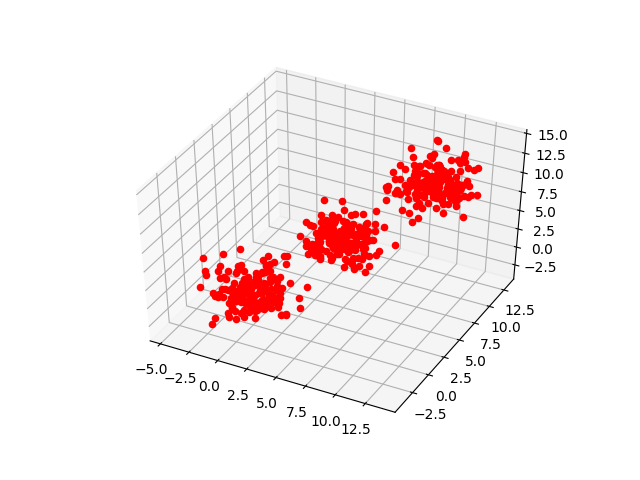
\includegraphics[width=1\linewidth]{images/figure_3}
  \caption{Synthetically generated 3-dimensional data}
  \label{fig:sub1}
\end{subfigure}%
\begin{subfigure}{.5\textwidth}
  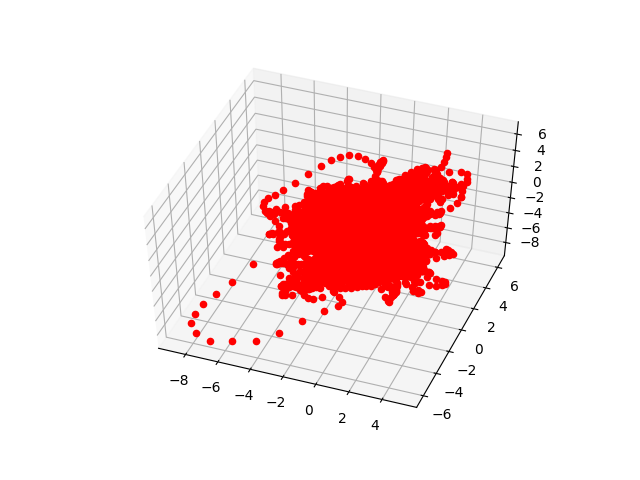
\includegraphics[width=1\linewidth]{images/figure_4}
  \caption{A subset of the 3-dimensional data found in the Heterogeneity Activity Recognition data set}
  \label{fig:sub2}
\end{subfigure}
\label{used data}
\end{figure}

\section{Performance}

All of the implemented algorithms have associated unit tests, which validate their correct execution when dealing with small, custom made input data sets. In order to examine the algorithms' performance when operating on larger, more substantial collections of data, the computing cluster, owned by the University of Glasgow School of Computing Science, was used. All of the presented experiments were carried out multiple time, thus the included runtime measurements are averaged over all attempts.

\subsection{Online K-Means using Grand Mean}

The non-streaming implementation of Online K-means was first tested using the synthetically generated data. The algorithm was able to correctly identify the used  cluster origin vectors in multiple scenarios with varying quantities of input points and observed dimensions. There were a few instances, however, where a poor choice for the \texttt{seed} parameter of the initial centroid selection function resulted in a unsatisfactory clustering. Although this is not due to a fault with the implementation, but rather an inherent weakness of the underlying algorithm.

To examine the algorithm's execution when clustering synthetic data in more detail,  one particular input set will be closely considered. The generated file consists of  100 thousand 3-dimensional data points clustered around the coordinates $(0,0,0)$, $(10,10,10)$ and $(20,20,20)$. When running the algorithm with the value of \texttt{K} set to $3$, the coordinates of the final cluster centroids are as follows: $(0.050,0.063,0.055)$, $(10.010,10.005,10.014)$ and $(20.002,20.0001,20.011)$. The respective WCSS value is also equal to 678737.057. These results are not surprising as identifying the centers of highly dissimilar clusters should not be problematic.

The implementation of standard K-Means that is present in MLlib was also run on the synthetic data. The algorithm was launched with 10 possible max iterations, K-Means++ as a way of initializing the centroids and \texttt{K} set to 3. The produced centroids had the following coordinates $(-0.013, -0.003, -0.009)$, $(9.998, 9.991, 10.001)$ and $(20.001, 19.999, 20.009)$. The value of WCSS in this case was 677308.787. This result is slightly better, however, it is also worth mentioning that the average runtime of the Online algorithm was 3.7 seconds and the  iterative one, with its present setting, had an average runtime of 17.9 seconds.

The two sets of results were also compared using Silhouette. Due to their similarity, the average score of each cluster in both models is around 0.805. By assigning such a high value to each cluster, Silhouette is also confirming that these center coordinates are nearly ideal.

\begin{figure}[H]
	\centering
    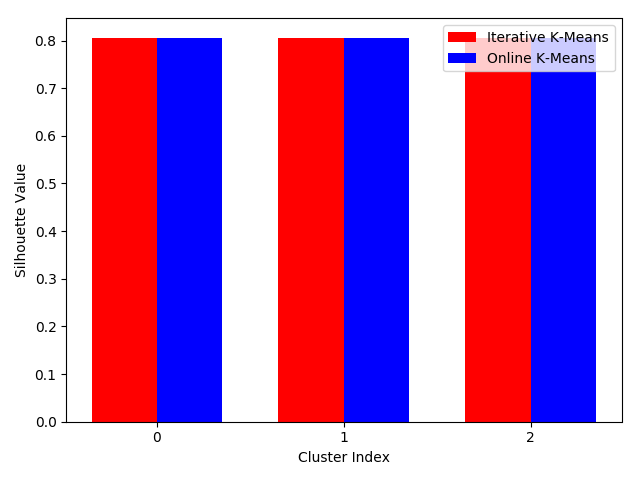
\includegraphics[width=0.7\textwidth]{images/result18}
    \caption{Silhouette values for the three cluster of synthetic data} 
    \label{fig:res18}
\end{figure}

To further inspect the differences between the two algorithms and the effects of different values of \texttt{K}, both algorithms were run 50 times, with an increasing value of \texttt{K} on each run. The resulting WCSS values were then plotted against each other.

\begin{figure}[H]
	\centering
    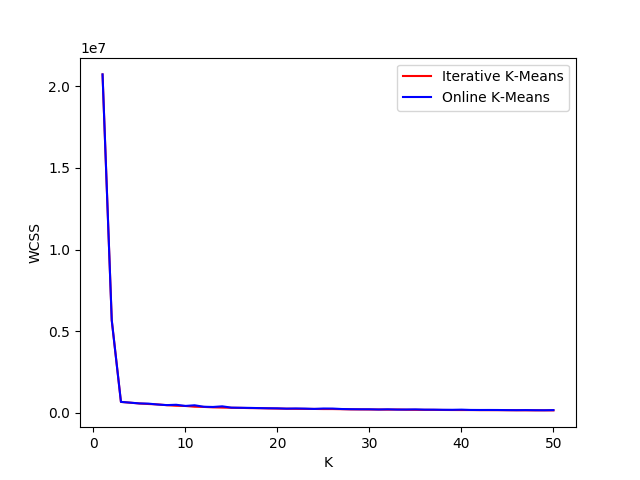
\includegraphics[width=0.68\textwidth]{images/result1}
    \caption{WCSS for increasing values of K -- clustering synthetic data} 
    \label{fig:res1}
\end{figure}

As expected, because the data set consists of 3 well defined clusters, the produced models with a number of clusters higher that 3 fail to significantly reduce the loss of the algorithm. Furthermore, because identifying a nearly ideal solution in the present dataset is so easy, the difference in the quality of each algorithm's model is almost unnoticeable.

The next experiment involves using input vectors from the \textit{Heterogeneity Activity Recognition Data Set}. Here the data once more consists of 100000 3-dimensional points, however, unlike the synthetic example, there are no highly dissimilar clusters. 

\begin{figure}[H]
	\centering
    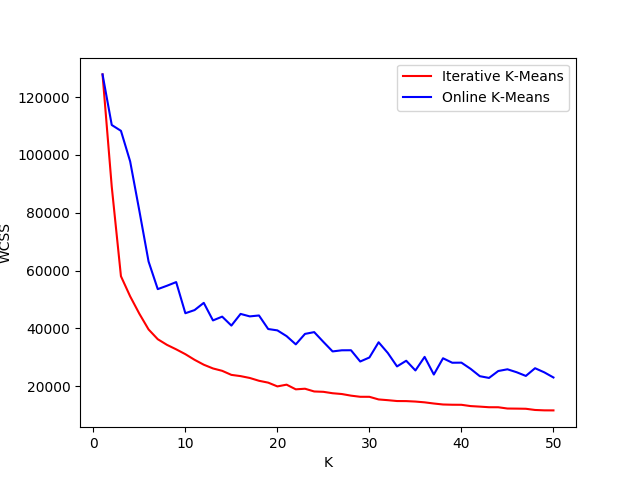
\includegraphics[width=0.68\textwidth]{images/result2}
    \caption{WCSS for increasing values of K -- clustering a subset of the HAR data set. Iterative K-Means set to use 10 max iterations and K-Means++ for centroid initialization. } 
    \label{fig:res2}
\end{figure}

These results seem to indicate that standard K-Means produces noticeably better results than Online K-Means. It is worth considering, however, that the implementation of standard K-Means is performing multiple iteration over the entire data (at most 10 in this example) and is also using K-Means++ to determine the starting coordinates of its centroids. Because of these model optimizations, performing all 50 clustering operations takes 5m 4.7s on average, where as Online K-Means takes only 59.7s. While the model is not of equally high quality, it was computed in less than one fifth of the time.

The obtained WCSS values for each execution of the two algorithms also indicate that a substantial decrease in the loss of the model does not occur after \texttt{K} is set to a value larger than 8. Because of this, the Silhouette scores of both models at \texttt{K} = 8 were measured. Here the average results are a lot worse than the ones obtained for clustering the synthetic data -- around 0.4 per cluster. This indicates that the models are reasonable but not perfect.

\begin{figure}[H]
	\centering
    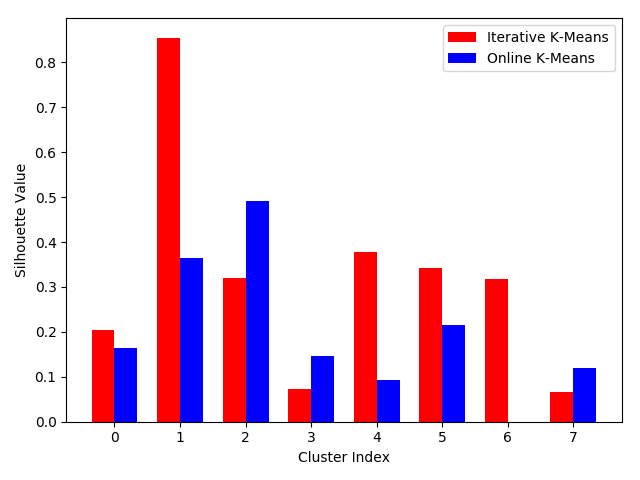
\includegraphics[width=0.75\textwidth]{images/result19}
    \caption{Silhouette values for 8 clusters of observations from the HAR data set.} 
    \label{fig:res19}
\end{figure}

To try and decrease the gap in execution time between the two algorithms, standard K-Means was ran on the same data set with 3 additional configurations:

\begin{enumerate}
\item 10 max iterations and random centroid initialization
\item 1 iteration over the data and K-Means++ for centroid initialization
\item 1 iteration over the data and random centroid initialization
\end{enumerate}

For the first two configurations, standard K-Means still manages to consistently produce a better model than Online K-Means -- although the WCSS curve for standard K-Means is noticeable less smooth (fig. \ref{fig:res3} and fig. \ref{fig:res4}). The average runtime of two variance has come down to  3m 44.2s for the first one and 2m 47.7s for the second one\footnote{The sum of the average run times for the two configurations is greater than 5m 4.7s, as without using K-Means++ for initialization, more of the 10 possible iterations need to be performed before the model converges.} -- these values are still orders of magnitude higher than 59.7s.

\begin{figure}[H]
	\centering
    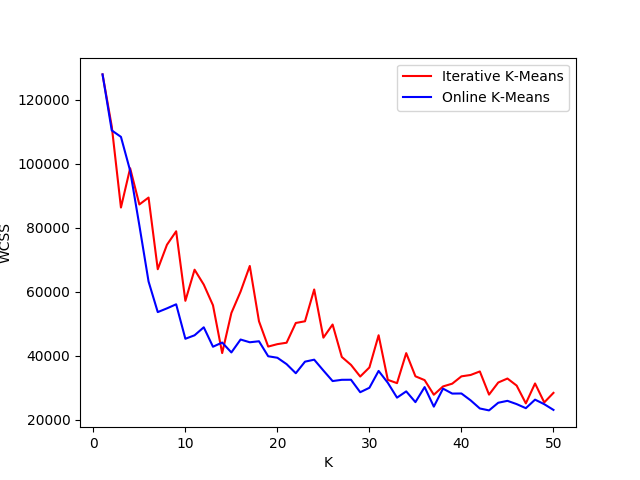
\includegraphics[width=0.96\textwidth]{images/result5}
    \caption{WCSS for increasing values of K -- clustering a subset of the HAR data set. Iterative K-Means set to use 1 iteration and random centroid initialization. }
    \label{fig:res5}
\end{figure}

Finally, when standard K-Means has been set to use only one iteration over the data  and to randomly initialize the starting coordinates of its centroids, does its execution time come close to that of Online K-Means -- 1m 8.4s. With all of its centroid optimization techniques disabled, however, the quality of the produced model by standard K-Means becomes highly erratic and of lower quality than that of Online K-Means.

The trend of Online K-Means providing a better quality model than standard K-Means, when operating with a nearly equivalent execution time, continues when looking at experiments that involve even larger quantities of data (fig. \ref{fig:res6} and fig. \ref{fig:res7}). In order to perform 50 clustering operations on the observations in the \textit{Individual household electric power consumption Data Set} (2 million 5-dimensional points) with incremental values of \texttt{K}, Online K-Means takes 13m 53s on average. Standard K-Means takes 1h 4m 12s when launched with 10 max iterations and K-Means++ for initialization,  and 14m 8s when using only 1 iteration and random centroid initialization.

Similar results are once again achieved when using the larges file from the \textit{Heterogeneity Activity Recognition Data Set} -- 14 million 3-dimensional data points (fig. \ref{fig:res8} and fig. \ref{fig:res9}). Online K-Means performs all 50 clustering operations in 45m 8s, standard K-Means takes 3h 31m 44s with 10 max iterations and K-Means++ for centroid initialization and 45m 3s with 1 iteration and random centroid initialization.

All of these measurements indicate that, while Iterative K-Means is able to generate better models by taking longer to process the data, Online K-Means is a preferred alternative when dealing with time-critical systems. Therefore, the created implementation offers a clear quality for performance trade-off which could be relevant for the purposes of the user.

\subsection{Online K-Means using Spark Streaming}

Testing the implementation of algorithms that rely on Spark Streaming proved more challenging, as it was first necessary to develop a small application that could simulate an input data stream. Unlike the first version of Online K-Means, where only a single file of N-dimensional vector data (stored on HDFS) was needed, for the purposes of streaming, the collection of data points first needed to be broken up into smaller chunks and later sent to the clustering algorithm, one chunk at a time. It is also required to set a time interval between each transfer.

This is done to enable the used \textit{discretized} stream to periodically feed the algorithm new observations in a similar meaner to a real use case, where a model needs to adapt to a live changing environment. Because of this method of operation, however, it is not possible to benchmark the processing speed of the algorithm, as its execution time is bottlenecked by the \textit{batch interval} specified by the Streaming Context.
 
The execution of Online K-Means with Spark Streaming was tested with both the synthetic and real data. In the first example, a collection of 100000 points clustered around the coordinates of (0,0,0), (10,10,10) and (20,20,20) was used, with each chunk of data sent to the algorithm containing 10000 points. The loss of the model (WCSS) was then recorded for incremental values of \texttt{K} and juxtaposed with the results returned by MLlib's Mini-batch K-Means (supplied with the same data).

\begin{figure}[H]
	\centering
    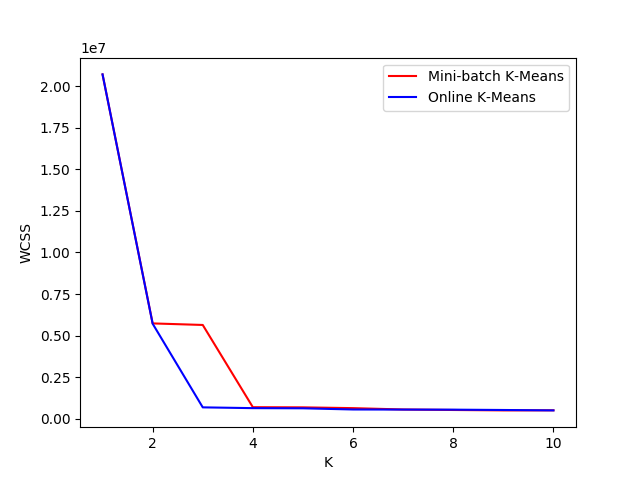
\includegraphics[width=0.83\textwidth]{images/result10}
    \caption{WCSS for increasing values of K -- clustering synthetic data} 
    \label{fig:res10}
\end{figure}

From the results, it is apparent that Online K-Means succeeded in finding the three appropriate centroid coordinates, when \texttt{K} was set to 3 -- afterwards the decrease in the model's loss is negligible. Mini-batch K-Means, on the other hand, did not manage to identify the cluster centers until \texttt{K} equaled 4. This is a result of poorly chosen starting coordinates -- Mini-batch K-Means does not provide an option to sample the data for centroid initialization and so a random values were used. By performing additional tests on synthetic data, it was discovered that both Mini-batch and Online K-Means have a tendency of producing low quality models, due to poor centroid initialization -- again a weakness of the underlying algorithms.

When the two streaming solutions were tested using observations from the  \textit{Heterogeneity Activity Recognition Data Set} (1 million points broken into chunks of 10000) with identical, manually selected, starting coordinates, they produced very similar results. This trend continued when testing with different input sets, indicating that, if the two algorithms have identical starting conditions, the quality of their produced models is nearly identical.

\begin{figure}[H]
	\centering
    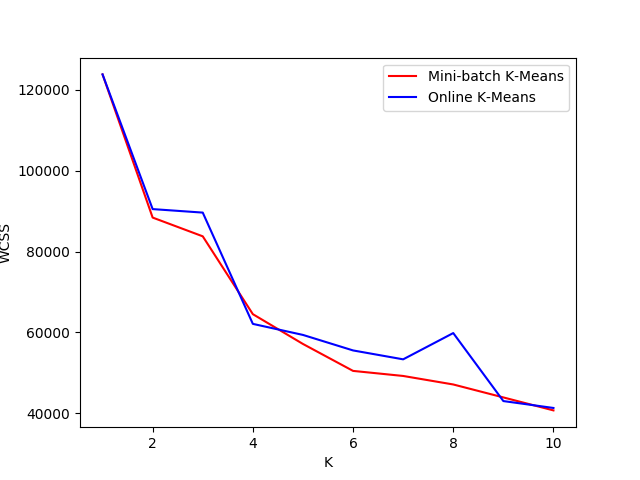
\includegraphics[width=0.82\textwidth]{images/result11}
    \caption{WCSS for increasing values of K -- clustering observations from the \textit{Heterogeneity Activity Recognition Data Set} with identical starting coordinates} 
    \label{fig:res11}
\end{figure}

The Silhouette values of the models produced by clustering the \textit{Heterogeneity Activity Recognition Data Set} with \texttt{K} set to 10 were also recorded (fig. \ref{fig:res20}). The average scores for each cluster is also very similar between the two algorithms.

\subsection{ART K-Means}

The implementation of ART K-Means was tested on synthetic and real data from the UCI Machine Learning Repository by also making use of the previously described stream simulating program. In this case, however, because of ART's unique input parameters and method of operation, there is no existing algorithm in MLlib that can be used for comparison purposes. Furthermore, since \texttt{K} is no longer a user supplied parameter, the loss of the model (WCSS) will be recorded for incremental values of the percentage of maximum \textit{vigilance}.

One experiment involved using the synthetic data set from before -- 100000 3-dimensional points, clustered around (0,0,0), (10,10,10) and (20,20,20), with each chunk from the simulated stream containing 10000 observations. Here, a high value for the percentage of the maximum vigilance value resulted in only one centroid being created at coordinates near (10,10,10). As this value was reduced, the model transitioned to having two centroids at roughly (5,5,5) and (15,15,15), until eventually the radius of the hyperspheres around the centroids became small enough to require three of them -- one at the center of each cluster. This stepwise shift in the number of centroids can be clearly seen when looking at a plot of the resulting models' loss.

\begin{figure}[H]
	\centering
    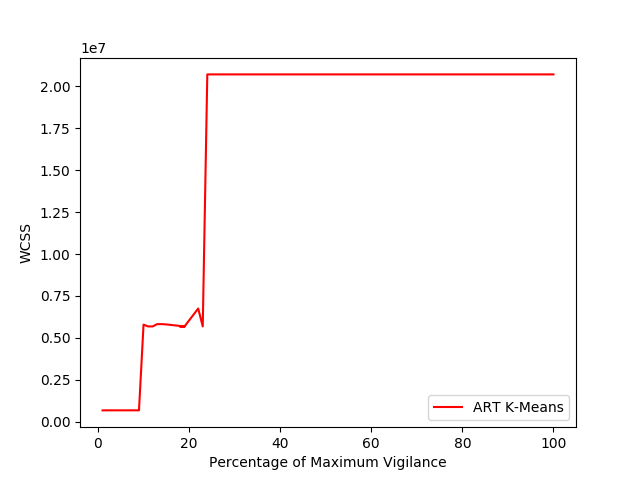
\includegraphics[width=0.83\textwidth]{images/result12}
    \caption{WCSS for increasing values of the percentage of maximum vigilance -- clustering synthetic data} 
    \label{fig:res12}
\end{figure}

It is worth pointing out that, in order to obtain a model with more than one centroid, a percentage smaller than 25 needs to be supplied. This is in fact normal behavior, caused by two different factors. Firstly, the three clusters are generated using a Gaussian function which occasionally creates points that are situated a fair distance away from their origin vector. Because of this, the values of the \textit{min} and \textit{max} vectors used by the algorithms are more extreme than [0,0,0] and [20,20,20] and so the resulting maximum possible vigilance becomes far greater. Secondly, when the collection of observations contains no outliers (e.g., points, whose normalized forms are situated near the corners of the unit hypercube) seemingly small vigilance values are enough to encompass all of the data(e.g., a hypersphere with a radius of 50\% max vigilance situates at the center of the unit hypercube).

When running ART K-Means on data from the \textit{Heterogeneity Activity Recognition} repository, a similar observation about the changing umber of centroids can be made (fig. \ref{fig:res13}). In this case, the clustering model contains more than one centroid when the percentage of max vigilance is less than 23\%. Then, the number of cluster centers rapidly grows to 11 at 5\% and 21 at 1\%.

One particular weakness of ART K-Means, that was identified during testing, is that
if the presented data contains an extreme outlier (e.g., a single point located a great distance from the majority of observations), a \textit{vigilance} percentage far smaller than 1\% would be required to obtain more than two clusters -- one for the outlier and one for the rest of the data. 

\subsection{SOM K-Means}

The SOM K-Means algorithm is fundamentally different to the rest of the implemented algorithms, as it not trying to identify the centers of existing data clusters but rather to form a topological map of the observed N-dimensional space. For this reason, methods like the Within-Cluster Sum of Squares formula and Silhouette are not adequate measurements of the quality of a produced model. Although, because the
purpose of this project is to provide scalable versions of proven machine learning algorithms, one way to evaluate SOM K-Means is to compare its output with that of a simple sequential version of the algorithm that does not use any of Spark's features. Using a third party library would not have been suitable, however, as the provided implementation would not be an exact sequential version of the algorithm implemented under Spark. Therefore, a sequential SOM K-Means was also created for comparison purposes.

SOM K-Means and its sequential variant were both tested with a variety of synthetic and real data input sets. Upon inspecting the values of neurons in the produced maps, there seemed to be a great deal of variance between the two algorithms -- neurons at identical indices in the two maps (trained on identical datasets) usually held completely different values. After a more detailed look at the overall structure of the maps, however, it became apparent that their neurons were largely grouped around the same regions, with a high density of observations, even if there wasn't a direct one-to-one correspondence between each neuron pair. 

The following is a visualization of the final coordinates of each neuron found in the 5x5 maps (with a neighborhood of size 1) obtained by running both the streaming and sequential versions of SOM K-Means on identical sets of synthetic and real data:

\begin{figure}[H]
\label{som-synth}
\begin{subfigure}{.5\textwidth}
  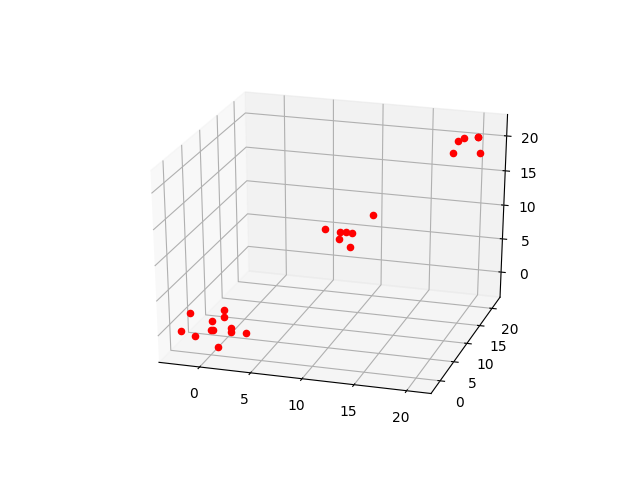
\includegraphics[width=0.95\linewidth]{images/result14}
  \caption{Sequential SOM K-Means}
  \label{fig:res14}
\end{subfigure}%
\begin{subfigure}{.5\textwidth}
  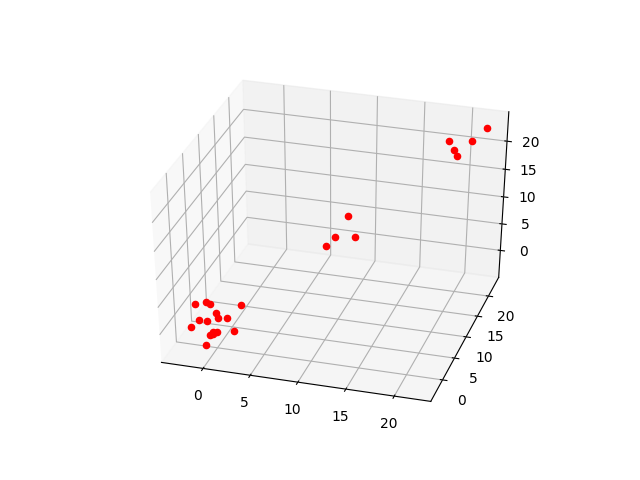
\includegraphics[width=0.95\linewidth]{images/result15}
  \caption{Streaming SOM K-Means}
  \label{fig:res15}
\end{subfigure}
\caption{The final coordinates of each neuron of a 5x5 map, trained using synthetic data}
\end{figure}

\begin{figure}[H]
\label{som-real}
\begin{subfigure}{.5\textwidth}
  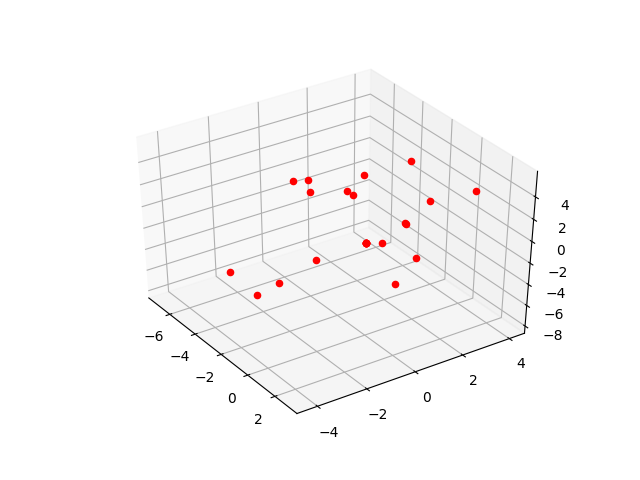
\includegraphics[width=0.95\linewidth]{images/result16}
  \caption{Sequential SOM K-Means}
  \label{fig:res16}
\end{subfigure}%
\begin{subfigure}{.5\textwidth}
  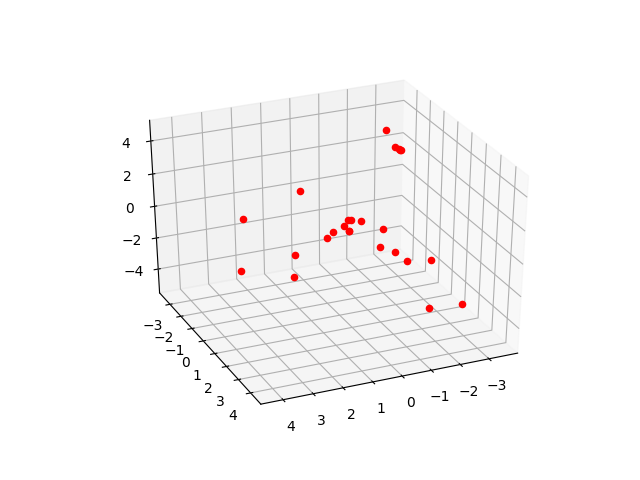
\includegraphics[width=0.95\linewidth]{images/result17}
  \caption{Streaming SOM K-Means}
  \label{fig:res17}
\end{subfigure}
\caption{The final coordinates of each neuron of a 5x5 map, trained using data from the HAR repository}
\end{figure}

%==============================================================================

\chapter{Conclusion}
\label{conclusion}

\section{Summary}

The aim of this project was to create an extension to the MLlib component of Apache Spark, by developing a variety of K-Means clustering algorithms that the framework does not currently support. The four implemented algorithms provide users with a plethora of options for clustering a set of observations that are not available in MLlib. Some have proven to be a superior choice when dealing with time-critical applications, while others are able to overcome the inherent weaknesses of standard K-Means thanks to their reliance on Spark Streaming and alternative models of operation. These qualities were exemplified while evaluating the algorithms with both synthetically generated data and samples from popular machine learning repositories.

\section{Future Work}

While the implemented algorithms present a solid foundation, there is a variety of possible extensions that could be made to enable users to further tailor the execution of clustering operations to better fit their use case. Some examples include:

\begin{itemize}
\item alternative methods for centroid initialization when using Spark Streaming -- e.g., running K-Means++ on a collection of the first few RDDs from the DStream
\item setting a lower bound on the possible centroid learning rate to increase the model's responsiveness to streamed data over a longer term
\item transition the implemented algorithms to use Spark's DataFrame API, which supports SQL queries
\end{itemize}

\section{Reflection}

Throughout the course of the project the author has gained substantial experience in understanding, implementing and evaluating machine learning algorithms. Achieving all this while also learning to use modern dig data processing and streaming technologies was a unique challenge that greatly enhances one's abilities to work in those fields. Additionally, the author has become more familiar with  contributing to an open source platform as well as writing functional code using the Scala programming language.

%==============================================================================

\bibliographystyle{plain}
\bibliography{l4proj}

%==============================================================================

\begin{appendices}

\chapter{Algorithm Execution DAGs}

This appendix contains the execution DAGs of all described algorithms -- images were taken from the Spark History Server

\section{Mini-batch K-Means Execution DAG}

\begin{figure}[H]
	\centering
    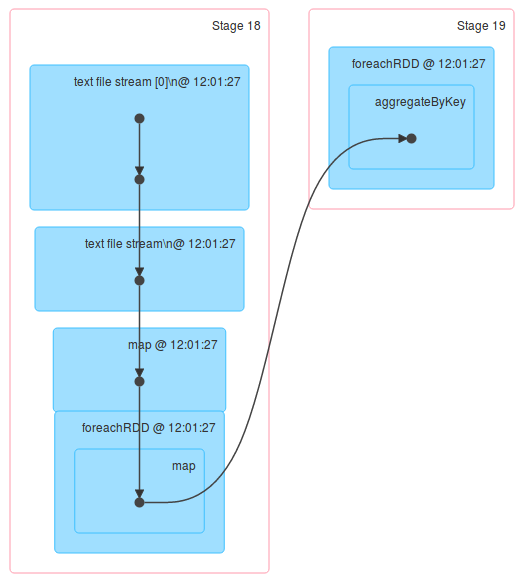
\includegraphics[width=0.70\textwidth]{images/DAG3}
    \label{fig:dag3}
\end{figure}

\section{Iterative K-Means Execution DAG}

\begin{figure}[H]
	\centering
    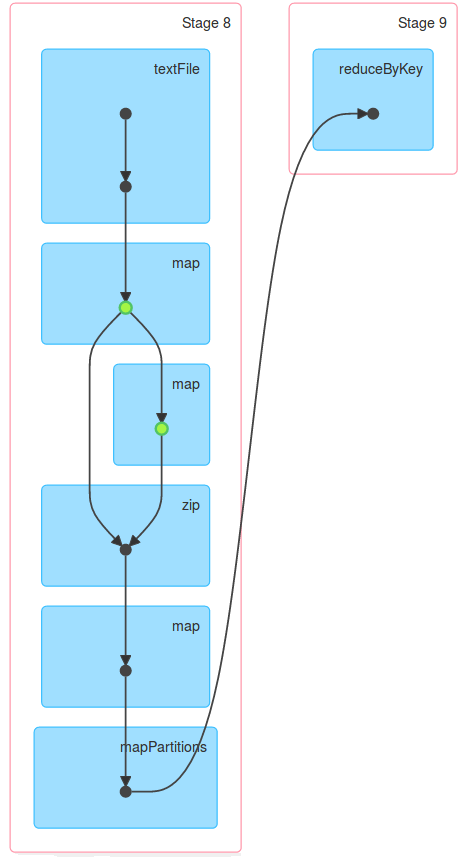
\includegraphics[width=0.70\textwidth]{images/DAG1}
    \label{fig:dag1}
\end{figure}

\section{K-Means++ Execution DAG}

\begin{figure}[H]
	\centering
    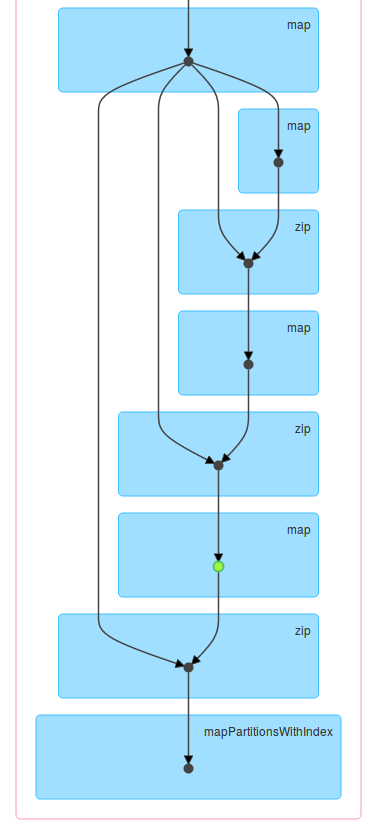
\includegraphics[width=0.60\textwidth]{images/DAG2}
    \label{fig:dag2}
\end{figure}

\section{Online K-Means using Grand Mean Execution DAG}

\begin{figure}[H]
	\centering
    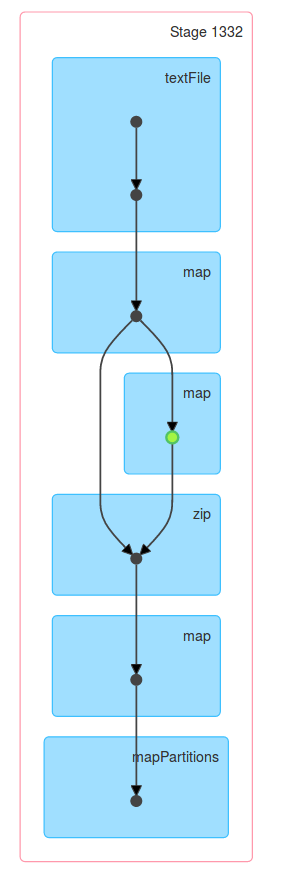
\includegraphics[width=0.40\textwidth]{images/DAG5}
    \label{fig:dag5}
\end{figure}

\section{Streaming Online K-Means Execution DAG}

\begin{figure}[H]
	\centering
    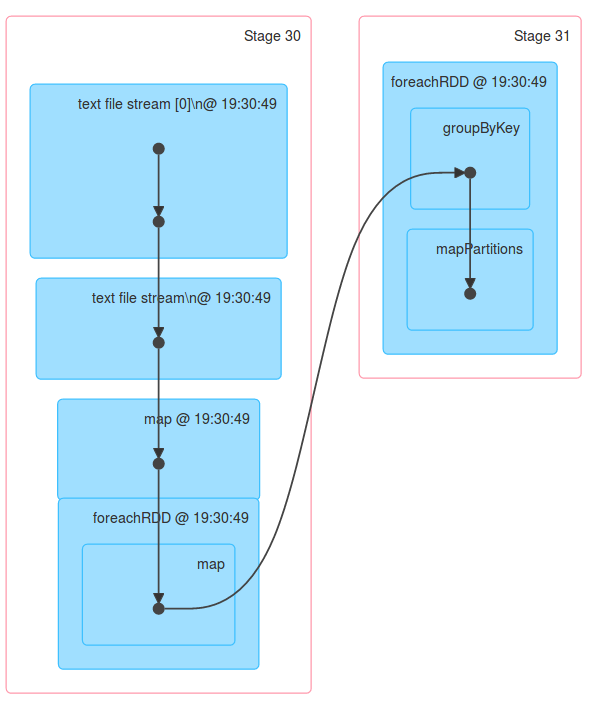
\includegraphics[width=0.80\textwidth]{images/DAG6}
    \label{fig:dag6}
\end{figure}

\section{ART K-Means Execution DAG}

\begin{figure}[H]
	\centering
    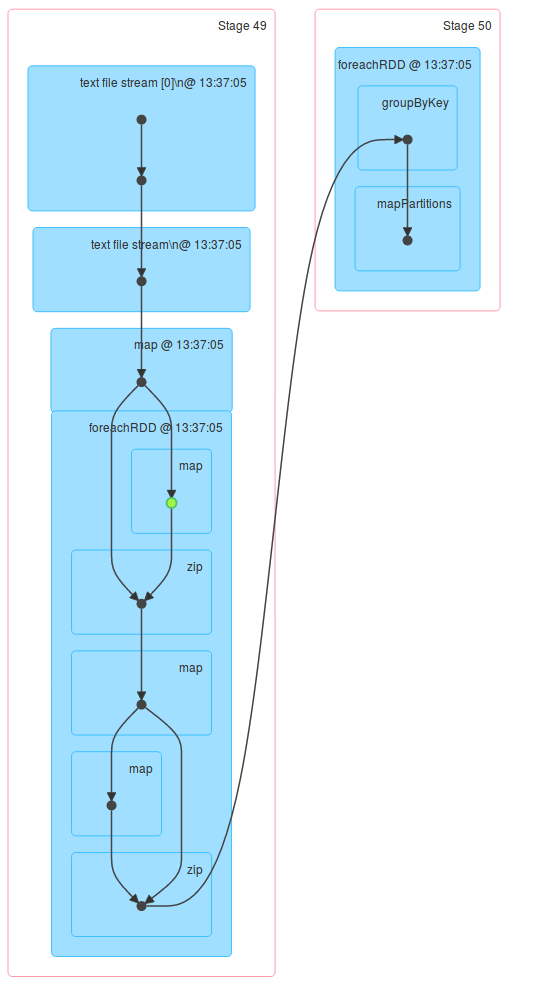
\includegraphics[width=0.73\textwidth]{images/DAG7}
    \label{fig:dag7}
\end{figure}

\section{SOM K-Means Execution DAG}

\begin{figure}[H]
	\centering
    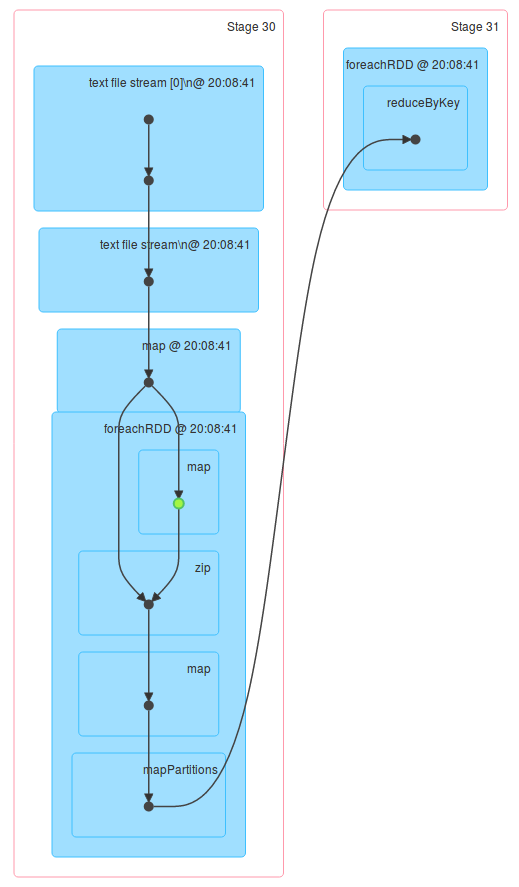
\includegraphics[width=0.75\textwidth]{images/DAG8}
    \label{fig:dag8}
\end{figure}

\chapter{Algorithm Evaluation Metrics}

\begin{figure}[H]
	\centering
    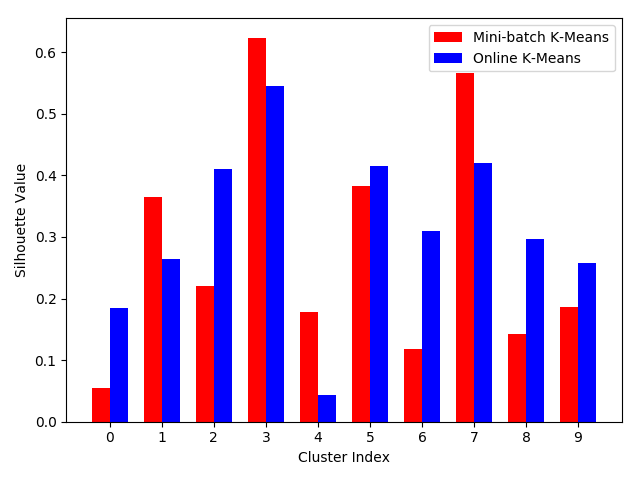
\includegraphics[width=1.0\textwidth]{images/result20}
    \caption{Silhouette values for 10 clusters of observations from the HAR data set.} 
    \label{fig:res20}
\end{figure}

\begin{figure}[H]
	\centering
    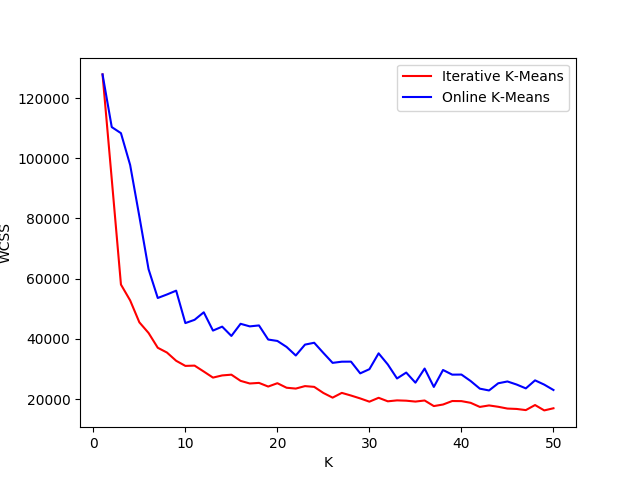
\includegraphics[width=0.825\textwidth]{images/result3}
    \caption{WCSS for increasing values of K -- clustering a subset of the HAR data set. Iterative K-Means set to use 10 max iterations and random centroid initialization. }
    \label{fig:res3}
\end{figure}

\begin{figure}[H]
	\centering
    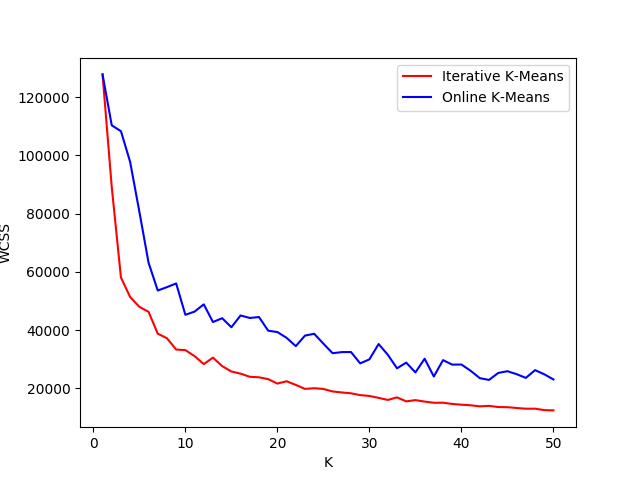
\includegraphics[width=0.825\textwidth]{images/result4}
    \caption{WCSS for increasing values of K -- clustering a subset of the HAR data set. Iterative K-Means set to use 1 iteration and K-Means++ for centroid initialization. } 
    \label{fig:res4}
\end{figure}

\begin{figure}[H]
	\centering
    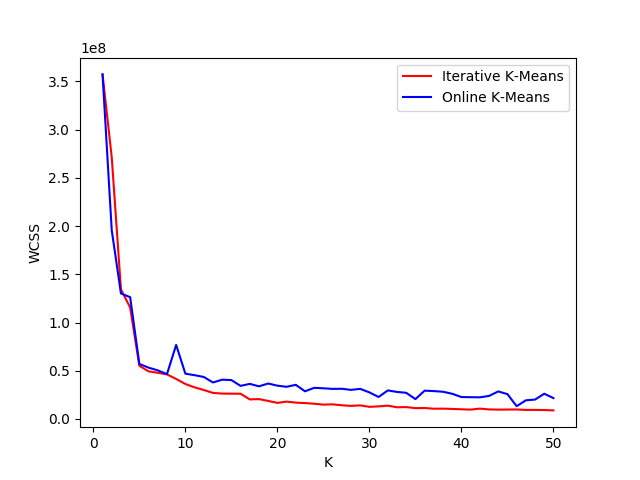
\includegraphics[width=0.825\textwidth]{images/result6}
    \caption{WCSS for increasing values of K -- clustering the entire IHEPC data set. Iterative K-Means set to use 10 max iterations and K-Means++ for centroid initialization. } 
    \label{fig:res6}
\end{figure}

\begin{figure}[H]
	\centering
    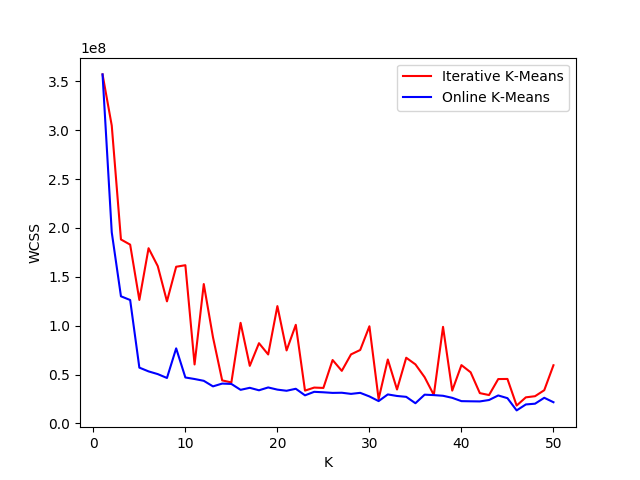
\includegraphics[width=0.825\textwidth]{images/result7}
    \caption{WCSS for increasing values of K -- clustering the entire IHEPC data set. Iterative K-Means set to use 1 iteration and random centroid initialization. }
    \label{fig:res7}
\end{figure}

\begin{figure}[H]
	\centering
    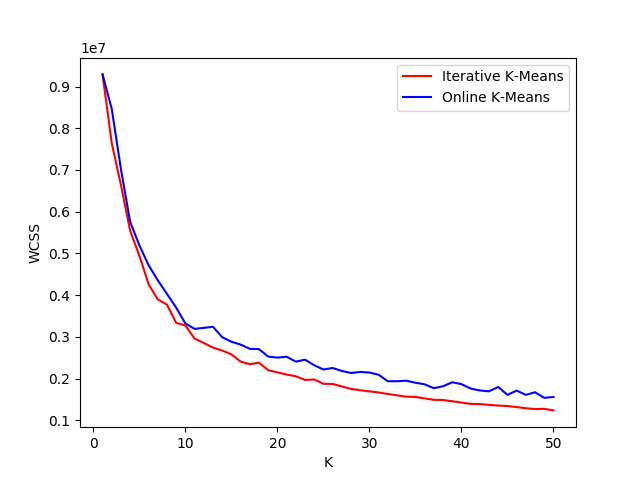
\includegraphics[width=0.825\textwidth]{images/result8}
    \caption{WCSS for increasing values of K -- clustering the larges file in the HAR data set. Iterative K-Means set to use 10 max iterations and K-Means++ for centroid initialization. } 
    \label{fig:res8}
\end{figure}

\begin{figure}[H]
	\centering
    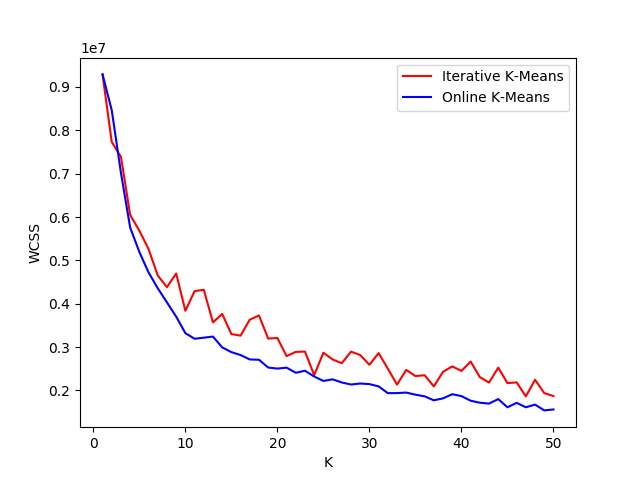
\includegraphics[width=0.825\textwidth]{images/result9}
    \caption{WCSS for increasing values of K -- clustering the larges file in the HAR data set. Iterative K-Means set to use 1 iteration and random centroid initialization. } 
    \label{fig:res9}
\end{figure}

\begin{figure}[H]
	\centering
    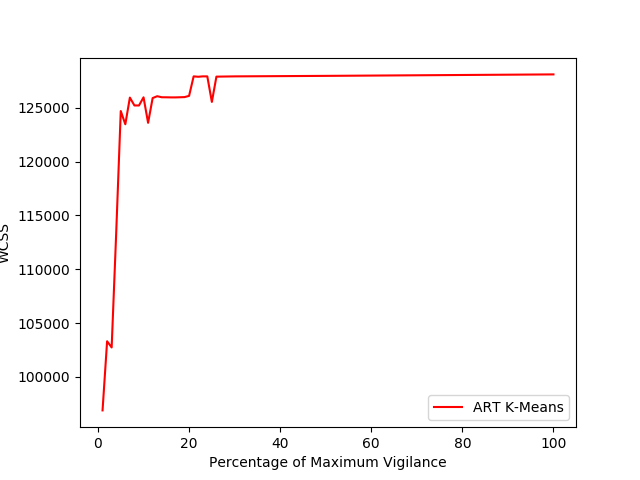
\includegraphics[width=1.0\textwidth]{images/result13}
    \caption{WCSS for increasing values of the percentage of maximum vigilance -- clustering observations from the HAR data set} 
    \label{fig:res13}
\end{figure}

\end{appendices}

\end{document}
